
% This is for rubber to remove slides.vrb automatically created by tikz
% rubber: watch $job.vrb
% rubber: clean $job.vrb
% rubber: rules rules.ini

\documentclass[xcolor=dvipsnames,12pt]{beamer}

% Include packages
\usepackage{colortbl}
\usepackage[absolute,overlay]{textpos}
\usepackage[normalem]{ulem}
\usepackage[override]{cmtt}
\usepackage{graphicx}
\usepackage{ifdraft}
\usepackage{tikz}
\usetikzlibrary{arrows,backgrounds}
\usepackage{xspace}
\usepackage{listings}
\lstset{language=Java,basicstyle=\small\ttfamily,lineskip=-0.25ex}

% Commands
\newcommand{\DSU}{{\sc Jvolve}\xspace}

% Include customized theme

\mode<beamer> {
  % But using Burnt orange instead of the blue used by that there. Changing
  % the beamercolor "structure" to burnt orange pretty much changes
  % everything. Really cool!!!
%   \definecolor{burntorange}{HTML}{CC5500}
%   \usecolortheme[named=burntorange]{structure}

%   The Copenhagen theme with innertheme [shadow=true] and rounded
%   \useinnertheme[shadow=true]{rounded}
  \usetheme{Madrid}
  \setbeamercolor{section in head/foot}{parent=palette tertiary}
  \setbeamercolor{subsection in head/foot}{parent=palette secondary}
  \setbeamercolor{date in head/foot}{parent=palette primary}
%   \setbeamersize{text margin left=1.5em,text margin right=1.5em}

%   The Warsaw theme and our customization
%   \usetheme{Warsaw}
%   \setbeamercolor*{palette quaternary}{use=structure,fg=white,bg=structure.fg!55!black}
%   \useoutertheme{split}

%   The Madrid theme and our customization
%   \usetheme[secheader]{Madrid}
%   \setbeamercolor*{subsection in head/foot}{parent=palette secondary}
%   \setbeamercolor*{palette quaternary}{use=structure,fg=white,bg=yellow}

  \setbeamercovered{transparent}

  \setbeamertemplate{footline}{%
   \begin{beamercolorbox}[wd=\paperwidth,ht=2.25ex,dp=1ex,right]{date in head/foot}%
     \usebeamerfont{date in head/foot}Slide \insertframenumber{}\hspace*{2ex}%
   \end{beamercolorbox}}

   \setbeamertemplate{sections/subsections in toc}[ball unnumbered]{}

   \setbeamertemplate{navigation symbols}{}
%   \setbeamertemplate{bibliography item}[text]
}

\mode<handout> {
  \usepackage{pgfpages}
  \pgfpagesdeclarelayout{6 on 1}
{
  \edef\pgfpageoptionheight{\the\paperwidth} % landscaped by default
  \edef\pgfpageoptionwidth{\the\paperheight}
  \def\pgfpageoptionborder{0pt}
  \def\pgfpageoptionfirstshipout{1}
}
{
  \pgfpagesphysicalpageoptions
  {%
    logical pages=6,%
    physical height=\pgfpageoptionheight,%
    physical width=\pgfpageoptionwidth,%
    current logical shipout=\pgfpageoptionfirstshipout%
  }
  \ifdim\paperheight>\paperwidth\relax
    % put side-by-side
    \pgfpageslogicalpageoptions{1}
    {%
      border shrink=\pgfpageoptionborder,%
      resized width=.5\pgfphysicalwidth,%
      resized height=\pgfphysicalheight,%
      center=\pgfpoint{.1667\pgfphysicalwidth}{.25\pgfphysicalheight}%
    }%
    \pgfpageslogicalpageoptions{3}
    {%
      border shrink=\pgfpageoptionborder,%
      resized width=.5\pgfphysicalwidth,%
      resized height=\pgfphysicalheight,%
      center=\pgfpoint{.5\pgfphysicalwidth}{.25\pgfphysicalheight}%
    }%
    \pgfpageslogicalpageoptions{5}
    {%
      border shrink=\pgfpageoptionborder,%
      resized width=.5\pgfphysicalwidth,%
      resized height=\pgfphysicalheight,%
      center=\pgfpoint{.8333\pgfphysicalwidth}{.25\pgfphysicalheight}%
    }%
    \pgfpageslogicalpageoptions{2}
    {%
      border shrink=\pgfpageoptionborder,%
      resized width=.5\pgfphysicalwidth,%
      resized height=\pgfphysicalheight,%
      center=\pgfpoint{.1667\pgfphysicalwidth}{.75\pgfphysicalheight}%
    }%
    \pgfpageslogicalpageoptions{4}
    {%
      border shrink=\pgfpageoptionborder,%
      resized width=.5\pgfphysicalwidth,%
      resized height=\pgfphysicalheight,%
      center=\pgfpoint{.5\pgfphysicalwidth}{.75\pgfphysicalheight}%
    }%
    \pgfpageslogicalpageoptions{6}
    {%
      border shrink=\pgfpageoptionborder,%
      resized width=.5\pgfphysicalwidth,%
      resized height=\pgfphysicalheight,%
      center=\pgfpoint{.8333\pgfphysicalwidth}{.75\pgfphysicalheight}%
    }%
  \else
    % stack on top of one another
    \pgfpageslogicalpageoptions{1}
    {%
      border shrink=\pgfpageoptionborder,%
      resized width=0.5\pgfphysicalwidth,%
      resized height=\pgfphysicalheight,%
      center=\pgfpoint{.25\pgfphysicalwidth}{.8333\pgfphysicalheight}%
    }%
    \pgfpageslogicalpageoptions{3}
    {%
      border shrink=\pgfpageoptionborder,%
      resized width=0.5\pgfphysicalwidth,%
      resized height=\pgfphysicalheight,%
      center=\pgfpoint{.25\pgfphysicalwidth}{.5\pgfphysicalheight}%
    }%
    \pgfpageslogicalpageoptions{5}
    {%
      border shrink=\pgfpageoptionborder,%
      resized width=0.5\pgfphysicalwidth,%
      resized height=\pgfphysicalheight,%
      center=\pgfpoint{.25\pgfphysicalwidth}{.1667\pgfphysicalheight}%
    }%
    \pgfpageslogicalpageoptions{2}
    {%
      border shrink=\pgfpageoptionborder,%
      resized width=0.5\pgfphysicalwidth,%
      resized height=\pgfphysicalheight,%
      center=\pgfpoint{.75\pgfphysicalwidth}{.8333\pgfphysicalheight}%
    }%
    \pgfpageslogicalpageoptions{4}
    {%
      border shrink=\pgfpageoptionborder,%
      resized width=0.5\pgfphysicalwidth,%
      resized height=\pgfphysicalheight,%
      center=\pgfpoint{.75\pgfphysicalwidth}{.5\pgfphysicalheight}%
    }%
    \pgfpageslogicalpageoptions{6}
    {%
      border shrink=\pgfpageoptionborder,%
      resized width=0.5\pgfphysicalwidth,%
      resized height=\pgfphysicalheight,%
      center=\pgfpoint{.75\pgfphysicalwidth}{.1667\pgfphysicalheight}%
    }%
  \fi
}

  \pgfpagesuselayout{8 on 1}[letterpaper,border shrink=1mm]
  \usetheme{default}
%   \setbeamertemplate{footline}[page number]
  \setbeamercolor{background canvas}{bg=black!5}
  \setbeamertemplate{footline}{%
   \begin{beamercolorbox}[wd=\paperwidth,ht=2.25ex,dp=1ex,right]{date in head/foot}%
     \usebeamerfont{date in head/foot}Slide \insertframenumber{}\hspace*{2ex}%
   \end{beamercolorbox}}
}

% If you have a file called "university-logo-filename.xxx", where xxx
% is a graphic format that can be processed by latex or pdflatex,
% resp., then you can add a logo as follows:

% \pgfdeclareimage[height=0.5cm]{university-logo}{university-logo-filename}
% \logo{\pgfuseimage{university-logo}}

% Delete this, if you do not want the table of contents to pop up at
% the beginning of each subsection:
% \AtBeginSubsection[]
% \AtBeginSection[]
% {
%   \begin{frame}<beamer>{Outline}
%     \tableofcontents[currentsection,currentsubsection]
%   \end{frame}
% }

% If you wish to uncover everything in a step-wise fashion, uncomment
% the following command: 

%\beamerdefaultoverlayspecification{<+->}


\title[Generating Heap Updates for Dynamic Software Updating]
{Generating Heap Updates for\\Dynamic Software Updating}

% \subtitle
% {Presentation Subtitle} % (optional)

\author[Suriya Subramanian]{%
Suriya Subramanian\inst{1} \and
Michael Hicks\inst{2}      \\ \and
Kathryn S\@. McKinley\inst{1}}
\institute[The University of Texas at Austin] % (optional, but mostly needed)
{
  \inst{1}Department of Computer Science\\
  The University of Texas at Austin
  \and
  \inst{2}Department of Computer Science\\
  University of Maryland, College Park
}

% \author[Suriya Subramanian]{Suriya Subramanian}
% \institute[]{Department of Computer Science\\
% The University of Texas at Austin}

\date[Short Occasion]
{January 14, 2010\\
Perpetually Available Software Systems\\Research Meeting}
\subject{}


\begin{document}


{
% UT seal got from http://www.utexas.edu/visualguidelines/vg_seals.html
\setbeamertemplate{navigation symbols}{}
\setbeamertemplate{headline}{}
\setbeamertemplate{footline}{}
% \mode<beamer>{
% \setbeamertemplate{background canvas}{{\color{bg}\vrule width 0\paperwidth height \paperheight}%
% 
\includegraphics[keepaspectratio=true,clip=true,trim=380pt 550pt 0pt 0pt]{theme/ut-seal}}
% }
\begin{frame}
  \titlepage
\end{frame}
}


% {
% \setbeamertemplate{headline}{}
% \setbeamertemplate{footline}{}
% \setbeamertemplate{navigation symbols}{}
% \begin{frame}
% \begin{block}{}
% \begin{quote}
% The only thing that is constant is change.\\
% \hfill Heraclitus of Ephesus
% \end{quote}
% \end{block}
% \end{frame}
% }

% \section{Introduction}
% \subsection{Motivation}
\begin{frame}{Motivation}%{A Sub-title is optional}
\begin{itemize}
\item Software applications change all the time
\item Deployed systems must be updated with bug fixes, new features
\item Updating typically involves: stop, apply patch, restart
% \vspace{1ex}
% \begin{center}\begin{Huge}Updating $\Rightarrow$ Downtime\end{Huge}\end{center}
\item Not desirable
  \begin{itemize}
    \item Safety concerns
    \item Revenue loss
    \item Inconvenience
  \end{itemize}
\end{itemize}
% \item Might not be affordable for some applications
%   \begin{itemize}
%   \item Applications that retain state that cannot be externalized
%   \end{itemize}
\end{frame}

\begin{frame}{Dynamic software updating}%{A Sub-title is optional}
\vspace*{-3mm}%
\begin{center}%
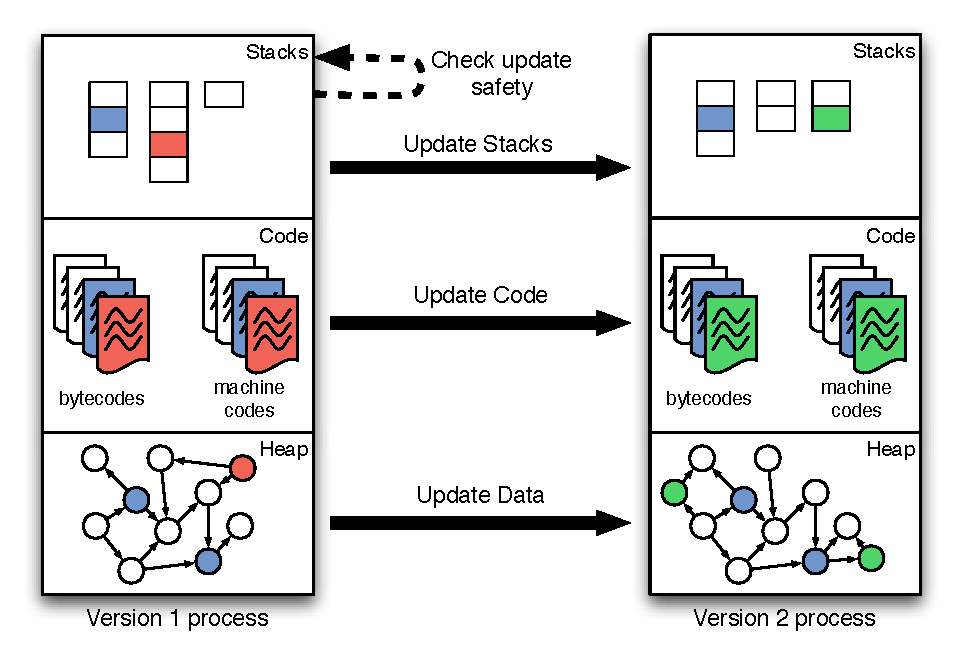
\includegraphics[scale=0.73]{images/process-state/both-process-state}%
\end{center}%
\end{frame}

\begin{frame}{Dynamic updating systems}%{A Sub-title is optional}
\begin{itemize}
\item Special-purpose architectures, application-specific solutions exist
\item General-purpose solutions gaining strength
  \begin{itemize}
  \item K42, Ksplice for OS updates
  \item Polus, Ginseng for C applications
  \end{itemize}
\item Not for managed languages
\end{itemize}
\end{frame}

% \begin{frame}{Motivation}%{A Sub-title is optional}
% \begin{itemize}
% \item Software applications change all the time
% \item Deployed systems need to be updated
% \item Some systems cannot afford downtime (safety concerns, revene loss),
% many systems perfer to avoid downtime (inconvenience)
% \item Stopping, updating and restarting deployed systems is not ideal
% \item Neither is delaying critical updates
% \end{itemize}
% \end{frame}

% \begin{frame}{Motivation}%{A Sub-title is optional}
% \begin{itemize}
% \item 75\% of downtime in high-availablity applications is for planned
% maintenance
% \uncover<2->{
% \item Personal operating system
% \item Enterprise applications
% \item Telecommunication, transportation systems
% % \uncover<3->{
% % \item Even a cache with lots of state
% %   \begin{itemize}
% %   \item LinkedIn.com architecture\footnote{\scriptsize{\url{http://hurvitz.org/blog/2008/06/linkedin-architecture}}}
% %   \item ``The Cloud'': In memory representation of the LinkedIn network graph
% %   \item Network size - 22M nodes, 120M edges
% %   \item Rebuilding an instance takes 8 hours
% %   \end{itemize}
% % }
% }
% \end{itemize}
% \end{frame}

% % \subsection{Solutions}
% \begin{frame}{Conventional solutions to avoid downtime}%{A Sub-title is optional}
% \begin{itemize}
% \item Move state out of the process, for instance databases
% \item Use multiple processes, and do a rolling update
% \end{itemize}
% \uncover<2>{
% \begin{itemize}
% \item Not always possible
% \item Restricted to specific application domains
% % \item DSU is a generic solution
% \end{itemize}
% }

% \begin{frame}{Dynamic Software Updating}%{A Sub-title is optional}
% Updating state of a process on the fly
% \begin{itemize}
% \item Special purpose techniques/architectures work, but we want a general
% solution
% \item 
% \end{itemize}
% \end{frame}

%   \begin{itemize}
%   \item State stored externally, for instance databases
%   \item Redundant systems: start a new process and stop this one
%   \item Not always possible
%   \end{itemize}
% \item<2-> Dynamic Software Updating (DSU)
%   \begin{itemize}
%     \item Update process state without restarting application
%     \item Non-redundant systems benefit as well
%     \item Decouples fault-tolerance from software updating
%   \end{itemize}
% \end{frame}

% \begin{frame}{Process state}%{A Sub-title is optional}
% \vspace*{-2ex}\includegraphics[scale=0.72]{images/process-state}
% \end{frame}

% \begin{frame}{DSU requirements}%{A Sub-title is optional}
% % \begin{center}
% % A Dynamic Software Updating solution should \emph{ideally} be
% % {\bf safe}, {\bf flexible}, and {\bf efficient}.
% % \end{center}
% \begin{description}
% \item[Safe] Updating is as correct as starting from scratch
% \item[Flexible] Support changes encountered in practice
% \item[Efficient] No performance impact
% \end{description}
% \end{frame}

% \begin{frame}{State of the art}%{A Sub-title is optional}
% Significant progress for C
% \begin{itemize}
% \item Server feature upgrades
%   \begin{itemize}
%   \item Ginseng \cite{neamtiu06dsu}
%   \item POLUS \cite{chen:icse07}
%   \end{itemize}
% \item Security patches: OPUS \cite{altekar05opus}
% \item Operating system upgrades
%   \begin{itemize}
%   \item K42 \cite{K42reconfig}
%   \item DynAMOS \cite{dynamos_eurosys_07}
%   \item LUCOS \cite{chen06vee}
%   \item Ksplice \cite{Ksplice}
%   \end{itemize}
% \end{itemize}
% % \item<2-> Primitive support for managed languages
% %   \begin{itemize}
% %   \item Very restrictive
% %   \item Space and time overheads
% %   \item Not proven on realistic applications
% %   \end{itemize}
% \end{frame}

% \begin{frame}{DSU opportunity for managed languages}%{A Sub-title is optional}
% DSU Solutions for C/C++ typically
% \begin{itemize}
% \item Require special compilation
% \item Statically/dynamically insert indirection for function calls
% \item Restrict structure updates, require extra allocation
% \item Impose space/time overheads on normal execution
% \item Make type-safety for updates difficult
% \item Not multi-threaded
% \end{itemize}
% \end{frame}

% \begin{frame}{Possible DSU solutions}%{A Sub-title is optional}
% Achieve DSU support by
% \begin{itemize}
% \item Making the application DSU-aware
% \item Special recompilation
% \item A class loader based colution 
% \item DSU support in the VM
% \end{itemize}
% \end{frame}

% \begin{frame}{Related work}%{A Sub-title is optional}
% \begin{itemize}
% \item Custom class loader solutions:\\Eisenbach and Barr, Milazzo et al.
% \item Source-to-source translation: Orso et al.
% \item VM-based solutions: JDrums, Dynamic Virtual Machine (DVM)
% \item In a persistent object store: Boyapati et al.
% \end{itemize}
% \uncover<2>{
% \begin{itemize}
% \item Limited, not flexible
% \item Restricted data-transformation model (like requiring {\em encapsulation} based
% on {\em ownership types})
% \item Overhead during normal execution
% \end{itemize}
% }
% \end{frame}

% \begin{frame}{Existing solutions for managed languages}%{A Sub-title is optional}
% \begin{itemize}
% \item VM-based solutions
%   \begin{itemize}
%   \item JDrums \cite{ritzau00dynamic}, DVM \cite{Mala00a}
%   \item Not well evaluated
%   \item Provide an interface similar to \DSU{}
%   \item Perform lazy updates
%   \item Overheads during normal execution
%   \end{itemize}
% \item Standard VM with DSU support
%   \begin{itemize}
%   \item DJVCS \cite{BarrE03}, DUSC \cite{orso:java}, \cite{Milazzo05updates}
%   \item Special classloaders, compilers
%   \item Very restrictive
%   \item Space/time overheads
%   \end{itemize}
% \end{itemize}
% 
% \end{frame}

% \begin{frame}{Related work}%{A Sub-title is optional}
% Nobody can beat us.
% \end{frame}

\begin{frame}{Our solution}%{A Sub-title is optional}
\begin{itemize}
\item \DSU{} - a Java Virtual Machine with DSU support
% \item Built on top of Jikes RVM, a Java-in-Java VM
\item Key insight: Extend existing VM services
%   \begin{itemize}
%   \item Classloading
%   \item Bytecode verification%\footnote{Jikes RVM does not have a bytecode verifier}
%   \item Thread synchronization
%   \item JIT Compilation
%   \item On-stack replacement
%   \item Garbage collection
%   \end{itemize}
\item No DSU-related overhead during normal execution
\item Support updates to real world applications
\begin{block}{}
\emph{Dynamic software updating in managed languages can be achieved in a
{\bf safe}, {\bf flexible} and {\bf efficient} manner by naturally extending existing VM
services.}
\end{block}

\begin{block}{}
\emph{DSU support should be a standard feature of future VMs.}
\end{block}
\end{itemize}
\end{frame}

% \begin{frame}{Contribution}%{A Sub-title is optional}
% \setbeamercovered{invisible}
% \begin{block}{}
% \emph{Dynamic software updating in managed languages can be achieved in a
% {\bf safe}, {\bf flexible} and {\bf efficient} manner by naturally extending existing VM
% services.}
% \end{block}
% 
% \begin{block}<2->{Corollary}
% \emph{DSU support should be a standard feature of future VMs.}
% \end{block}
% \end{frame}


\section{\DSU}
\ShowTOC[currentsection]
\subsection{Developer's view}

\begin{frame}{Developer's view of \DSU{}}%{A Sub-title is optional}
\begin{center}
\includegraphics[width=0.84\paperwidth]{system.pdf}
\end{center}
\end{frame}

\begin{frame}{Division of Labor}%{A Sub-title is optional}
\begin{itemize}
\item Developer
  \begin{itemize}
  \item Write the old and new versions
  \item Write class/object transformation functions for classes that
        changed (optional)
  \item Testing (both the application and the update)
  \end{itemize}
\item \DSU{} system
  \begin{itemize}
  \item Update Preparation Tool (UPT) compares versions and presents the
        update to the \DSU{} VM.
  \item \DSU{} VM handles the update
  \end{itemize}
\end{itemize}
\end{frame}

\begin{frame}{Supported updates}%{A Sub-title is optional}
\begin{itemize}
\item Changes within the body of a method
\item Class signature updates
  \begin{itemize}
  \item Add, remove, change the type signature of fields and methods
  \end{itemize}
\item Changes can occur at any level of the class hierarchy
\end{itemize}
\end{frame}

\newcommand{\ExampleCodeSize}{footnotesize}
\begin{frame}[fragile,shrink=5]{Example of an update (JavaEmailServer)}%{A Sub-title is optional}
\begin{\ExampleCodeSize}
\begin{verbatim}
  public class User {
    private String username, domain, password;
    private String[] forwardAddresses;
    public String[] getForwardedAddresses() {...}
    public void setForwardedAddresses(String[] f) {...}
  }

  public class ConfigurationManager {
    private User loadUser(...) {
       ...
       User user = new User(...);
       String[] f = ...;
       user.setForwardedAddresses(f);
       return user;
    }
  }




\end{verbatim}
\end{\ExampleCodeSize}
\end{frame}

% \begin{frame}[fragile,shrink=5]{Example of an update (JavaEmailServer)}%{A Sub-title is optional}
% \begin{\ExampleCodeSize}
% \begin{semiverbatim}
% public class User \{
%   private String username, domain, password;
%   private \sout{String[]} EmailAddress[] forwardAddresses;
%   public \sout{String[]} EmailAddress[] getForwardedAddresses() \{...\}
%   public void setForwardedAddresses(\sout{String[]} EmailAddress[] f) \{...\}
% \}
% 
% public class ConfigurationManager \{
%   private User loadUser(...) \{
%      ...
%      User user = new User(...);
%      \sout{String[]} EmailAddress[] f = ...;
%      user.setForwardedAddresses(f);
%      return user;
%   \}
% \}
% 
% \end{semiverbatim}
% \end{\ExampleCodeSize}
% \end{frame}

\begin{frame}[fragile,shrink=5]{Example of an update (JavaEmailServer)}%{A Sub-title is optional}
\newcommand{\removed}[1]{\textcolor{red}{- #1}}
\newcommand{\addedxx}[1]{\textcolor{OliveGreen}{+ #1}}
\begin{\ExampleCodeSize}
\begin{semiverbatim}
  public class User \{
    private String username, domain, password;
\removed{  private String[] forwardAddresses;}
\removed{  public String[] getForwardedAddresses() \{...\}}
\removed{  public void setForwardedAddresses(String[] f) \{...\}}
\addedxx{  private EmailAddress[] forwardAddresses;}
\addedxx{  public EmailAddress[] getForwardedAddresses() \{...\}}
\addedxx{  public void setForwardedAddresses(EmailAddress[] f) \{...\}}
  \}

  public class ConfigurationManager \{
    private User loadUser(...) \{
       ...
       User user = new User(...);
\removed{     String[] f = ...;}
\addedxx{     EmailAddress[] f = ...;}
       user.setForwardedAddresses(f);
       return user;
    \}
  \}
\end{semiverbatim}
\end{\ExampleCodeSize}
\end{frame}

\begin{frame}{Object Transformers}%{A Sub-title is optional}
\begin{itemize}
\item ``Transform'' objects to correspond to the new version
\item A function specified as part of the new version of a class
\item Accepts old object and new object as parameters
\item VM runs a default transformer that copies old fields and initializes
new ones to \texttt{null}
\end{itemize}
\end{frame}

\begin{frame}[fragile,shrink=5]{Object Transformers}%{A Sub-title is optional}
\mode<beamer> {
\begin{textblock*}{46mm}[0,0](79mm,20mm)
\begin{block}{}
Stub generated by UPT for the old version
\end{block}
\end{textblock*}
\begin{textblock*}{46mm}[0,0](79mm,48mm)
\begin{block}{}
Default transformer copies old fields, initializes new ones to
\texttt{null}
\end{block}
\end{textblock*}
}
\begin{small}
\begin{semiverbatim}
public class old_User \{
  public String username, domain, password;
  public String[] forwardAddresses;
\}
public class User \{
  ...
  public static void jvolve_class() \{ ... \}
  public static void jvolve_object(User to, old_User from) \{
    to.username = from.username;
    to.domain = from.domain;
    to.password = from.password;
    to.forwardAddresses = null;
    \uncover<2>{int l = from.forwardAddresses.length;
    to.forwardAddresses = new EmailAddress[l];
    for (int i = 0; i < l; i++)
      to.forwardAddresses[i] =
       new EmailAddress(from.forwardAddresses[i]);
}\}\}

\end{semiverbatim}
\end{small}
\end{frame}

% \newcommand{\JvolveTimeLine}[5]{
\begin{center}
\begin{tikzpicture}[auto]
  \tikzstyle{block}=[
    font=\tiny,
    rectangle,
    draw=structure.fg,
    thick,
    text width=1.2cm,
    text badly centered,
    rounded corners,
    minimum height=2em,
  ]
  \tikzstyle{current}=[fill=structure.fg!20, ]
  \tikzstyle{line}=[draw, thick, -latex',]
  \tikzstyle{every path}=[line]
  \matrix [column sep=5mm,row sep=7mm,ampersand replacement=\&] {
    \node [block,#1] (0) {\hyperlink{offline}{Offline tool}};          \&
    \node [block,#2] (1) {\hyperlink{suspend}{Suspend application}};   \&
    \node [block,#3] (2) {\hyperlink{classload}{Load new classes}};    \&
    \node [block,#4] (3) {\hyperlink{transform}{Transform objects}};   \&
    \node [block,#5] (4) {Resume application};                         \\
  };
  \path (0) -- (1);
  \path (1) -- (2);
  \path (2) -- (3);
  \path (3) -- (4);
\end{tikzpicture}
\end{center}
}


\subsection{VM Implementation}
% \ShowTOC

% \begin{frame}[fragile]{Update process}%{A Sub-title is optional}
% \JvolveTimeLine{}{}{}{}{}
% \begin{itemize}
% \item Offline Update Preparation Tool (UPT)
% \item \DSU{} VM
%   \begin{itemize}
%   \item Reach a safe point in the VM%(thread synchronization)
%   \item Install new classes%(classloader)
%   \item Transform objects to new definition%(garbage collector)
%   \item Resume execution
%   \end{itemize}
% \end{itemize}
% \end{frame}

%L  \begin{frame}[t,fragile,label=offline]{Update Preparation Tool}%{A Sub-title is optional}
%L  % \vspace{-2ex}
%L  \JvolveTimeLine{current}{}{}{}{}
%L  % \vspace{-2ex}
%L  \begin{itemize}
%L  \item Uses jclasslib\footnote{\url{http://jclasslib.sourceforge.net}}, a
%L  bytecode modification library
%L  \item Compares bytecodes of the two versions
%L  % \item Categorizes changes into
%L  %   \begin{description}
%L  %   \item[Updated classes] Classes that add, remove, change signature of fields
%L  %                        or methods
%L  %   \item[Updated methods] Changes within a method body. Only the method has
%L  %                         to be loaded/updated
%L  %   \item[Indirect updates] No change to method, but refers to changed
%L  %                           classes
%L  %   \end{description}
%L  \item Generates old version stubs and default object transformers
%L  \end{itemize}
%L  \end{frame}
%L
%L  \begin{frame}[t,fragile]{Compiling transformation functions}%{A Sub-title is optional}
%L  \begin{itemize}
%L  \item All transformers specified in a separate source file
%L  \item Class transformers  \\ \hspace{6ex} {\footnotesize {\tt jvolveClass(ClassName unused)}}
%L  \item Object transformers \\ \hspace{6ex} {\footnotesize {\tt jvolveObject(old\_ClassName from, ClassName to)}}
%L  \item Compiled specially by a JastAddJ extension to the Java language
%L  \item Ignores access protection and allows assigning to {\tt final} fields
%L  \end{itemize}
%L  \end{frame}

%L% \begin{frame}[t,fragile,label=offline]{Update Preparation Tool}%{A Sub-title is optional}
%L% % \vspace{-2ex}
%L% \JvolveTimeLine{current}{}{}{}{}
%L% % \vspace{-2ex}
%L% \begin{itemize}
%L% \item Uses jclasslib\footnote{\url{http://jclasslib.sourceforge.net}}, a
%L% bytecode modification library
%L% \item Generates old version stubs and default object transformers
%L% \item Compiled specially by a JastAddJ extension to the Java language
%L% \begin{itemize}
%L%   \item Ignores access protection and allows assigning to {\tt final} fields
%L% \end{itemize}
%L% \end{itemize}
%L% \end{frame}

\begin{frame}[t,fragile,label=suspend]{Safe point for the update}%{A Sub-title is optional}
\JvolveTimeLine{}{current}{}{}{}
\begin{itemize}
\item Update must be atomic
\item Updates happen at ``safe points''\\
      (VM yield points with restriction on what methods can be on stack)
\item Extend the thread scheduler to suspend all application threads
\item Examine all stacks, ensure no restricted methods on stack and perform
      the update
\end{itemize}
\end{frame}

\begin{frame}[t,fragile]{Restricted methods}%{A Sub-title is optional}
\begin{enumerate}[(1)]
\item Methods changed by the update
\item Methods whose bytecode is unchanged, but compiled representation is
      changed by the update
  \begin{itemize}
  \item Offsets of fields and methods hard-coded in machine code
  \item Inlined callees may have changed
  \end{itemize}
\item Methods identified by the user as unsafe based on semantic
information about the application
\end{enumerate}
\uncover<2>{
Handling restricted methods
\begin{itemize}
\item \emph{On-stack replace} baseline-compiled category (2) methods
\item Do not allow (1) and (3) to be active on stack, install a return
      barrier for such methods
\end{itemize}
}
\end{frame}

\begin{frame}{Handling restricted methods}%{A Sub-title is optional}
\vspace*{-2mm}%
\begin{center}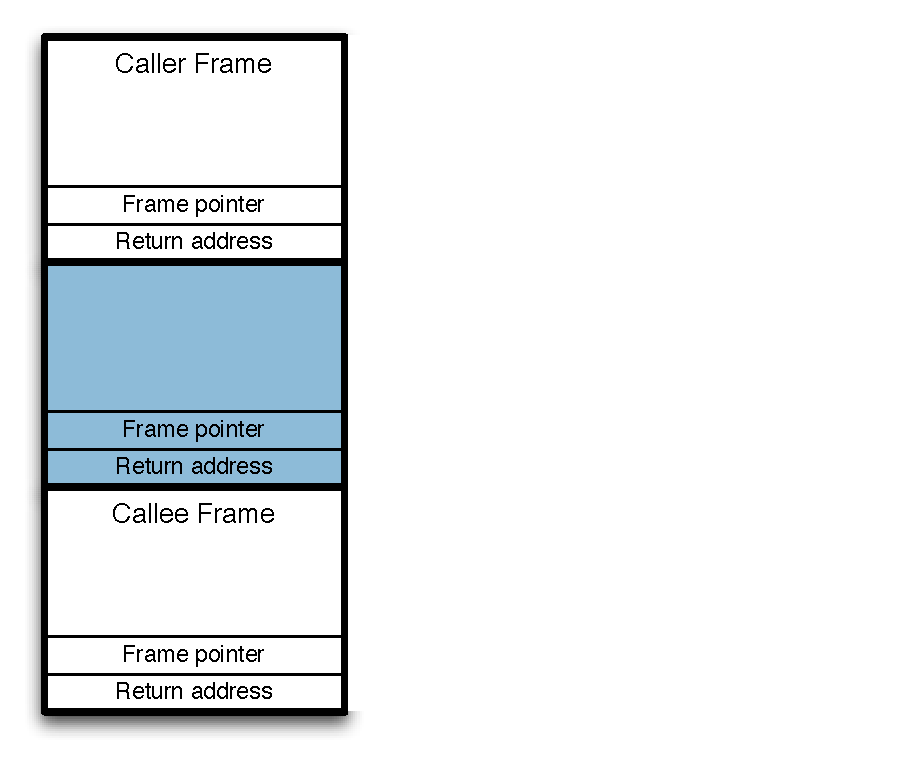
\includegraphics[scale=0.62]{images/stack-smash/stack-frames-overview}\end{center}
\end{frame}

\begin{frame}{Performing On-stack replacement}%{A Sub-title is optional}
\vspace*{-2mm}%
\begin{center}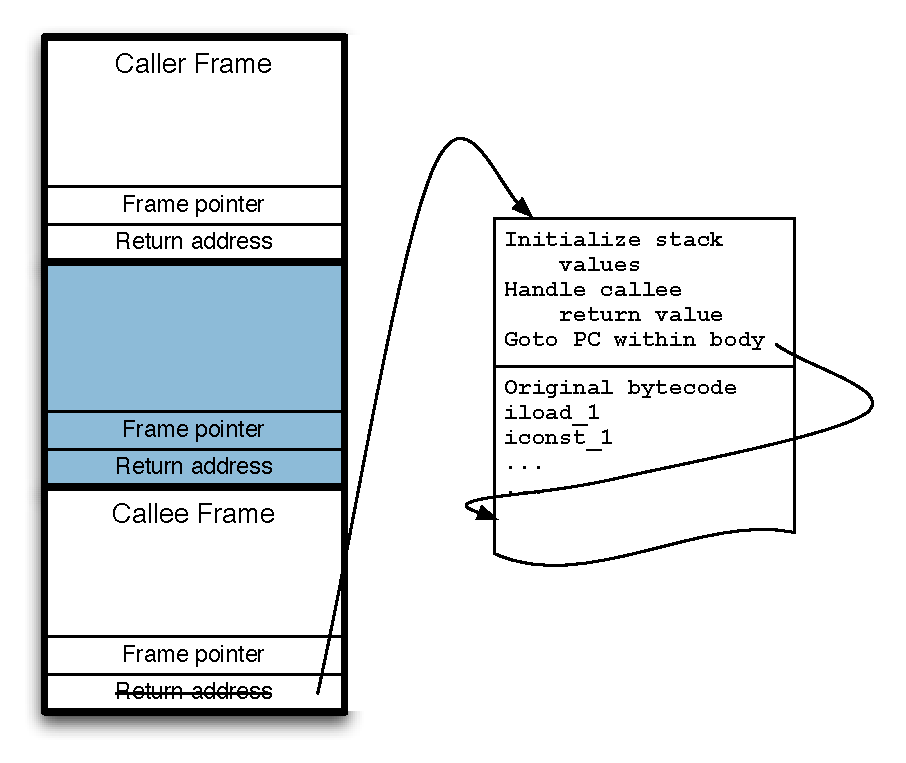
\includegraphics[scale=0.62]{images/stack-smash/osr-overview}\end{center}
\end{frame}

\begin{frame}{Installing return barrier for DSU}%{A Sub-title is optional}
\vspace*{-2mm}%
\begin{center}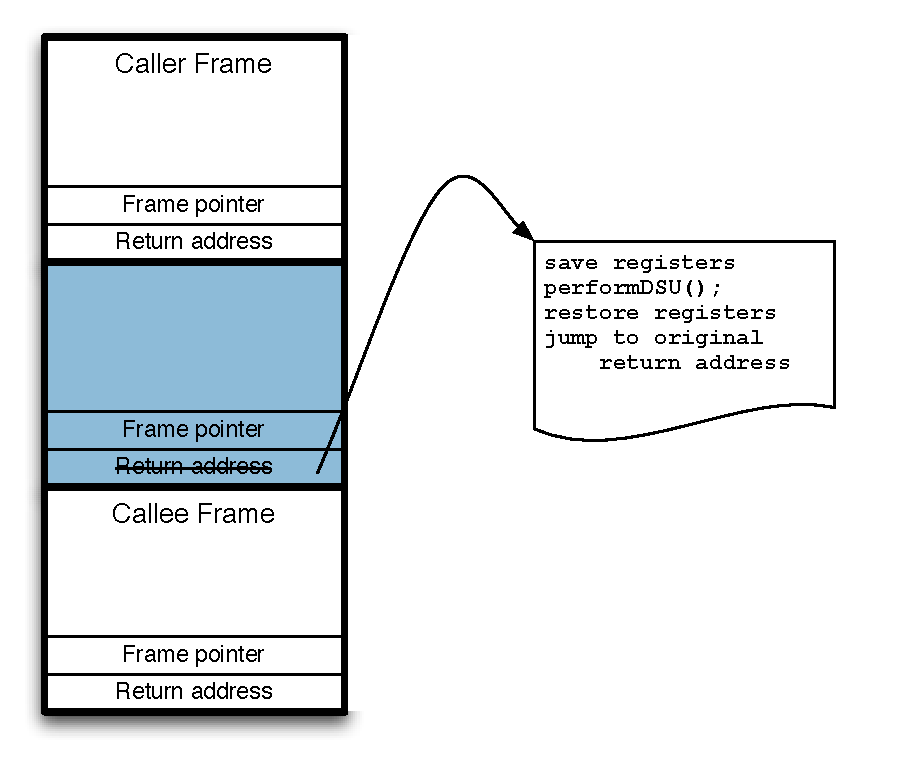
\includegraphics[scale=0.62]{images/stack-smash/return-barrier-overview}\end{center}
\end{frame}

\begin{frame}{Reaching a safe point}%{A Sub-title is optional}
\hspace*{-3mm}
\scalebox{0.44}{%
\uncover<1>{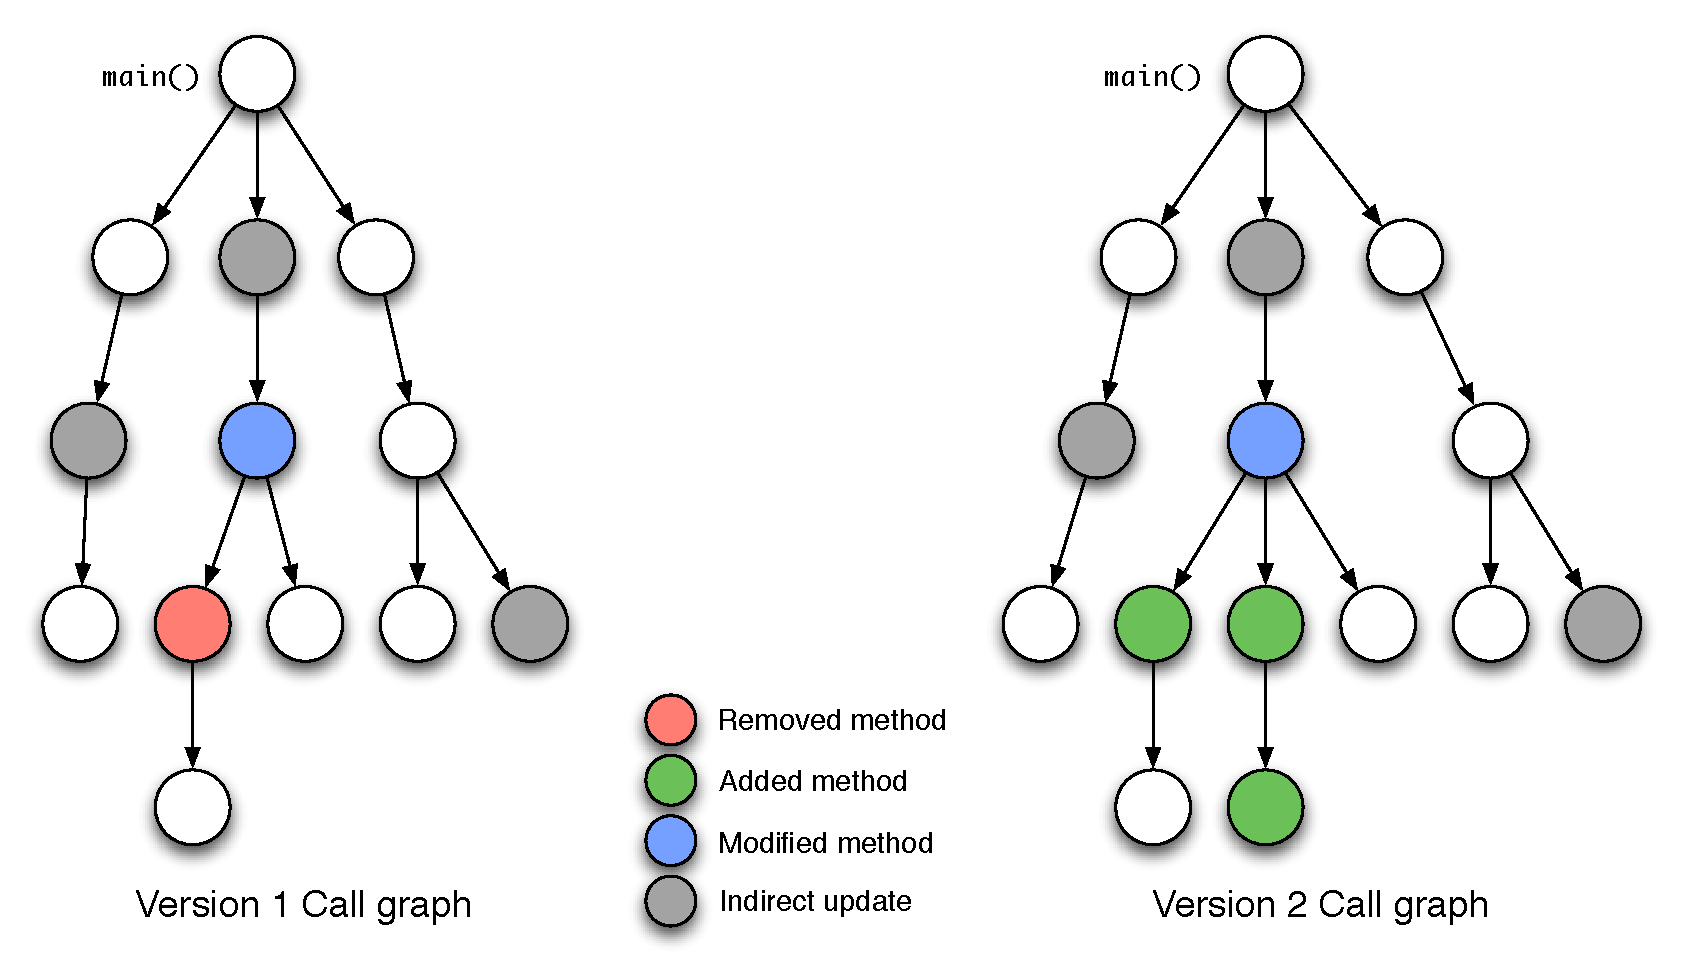
\includegraphics{images/safe-point-call-graph/both-call-graphs-1}}%
\uncover<2>{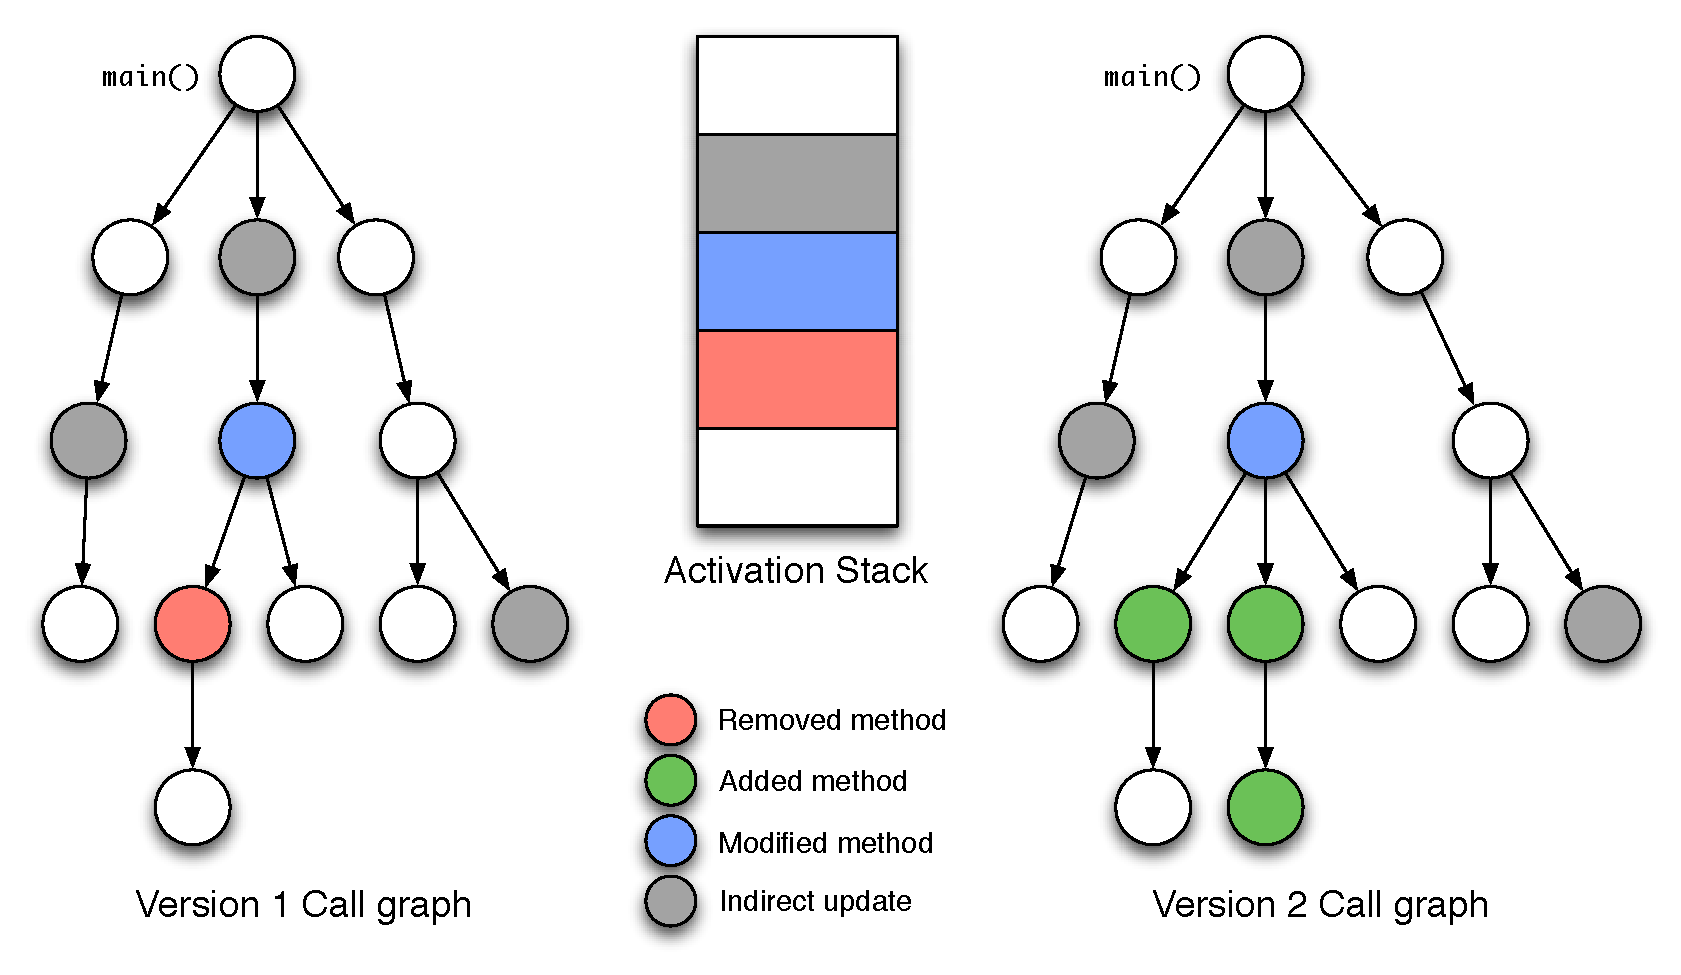
\includegraphics{images/safe-point-call-graph/both-call-graphs-2}}%
\uncover<3>{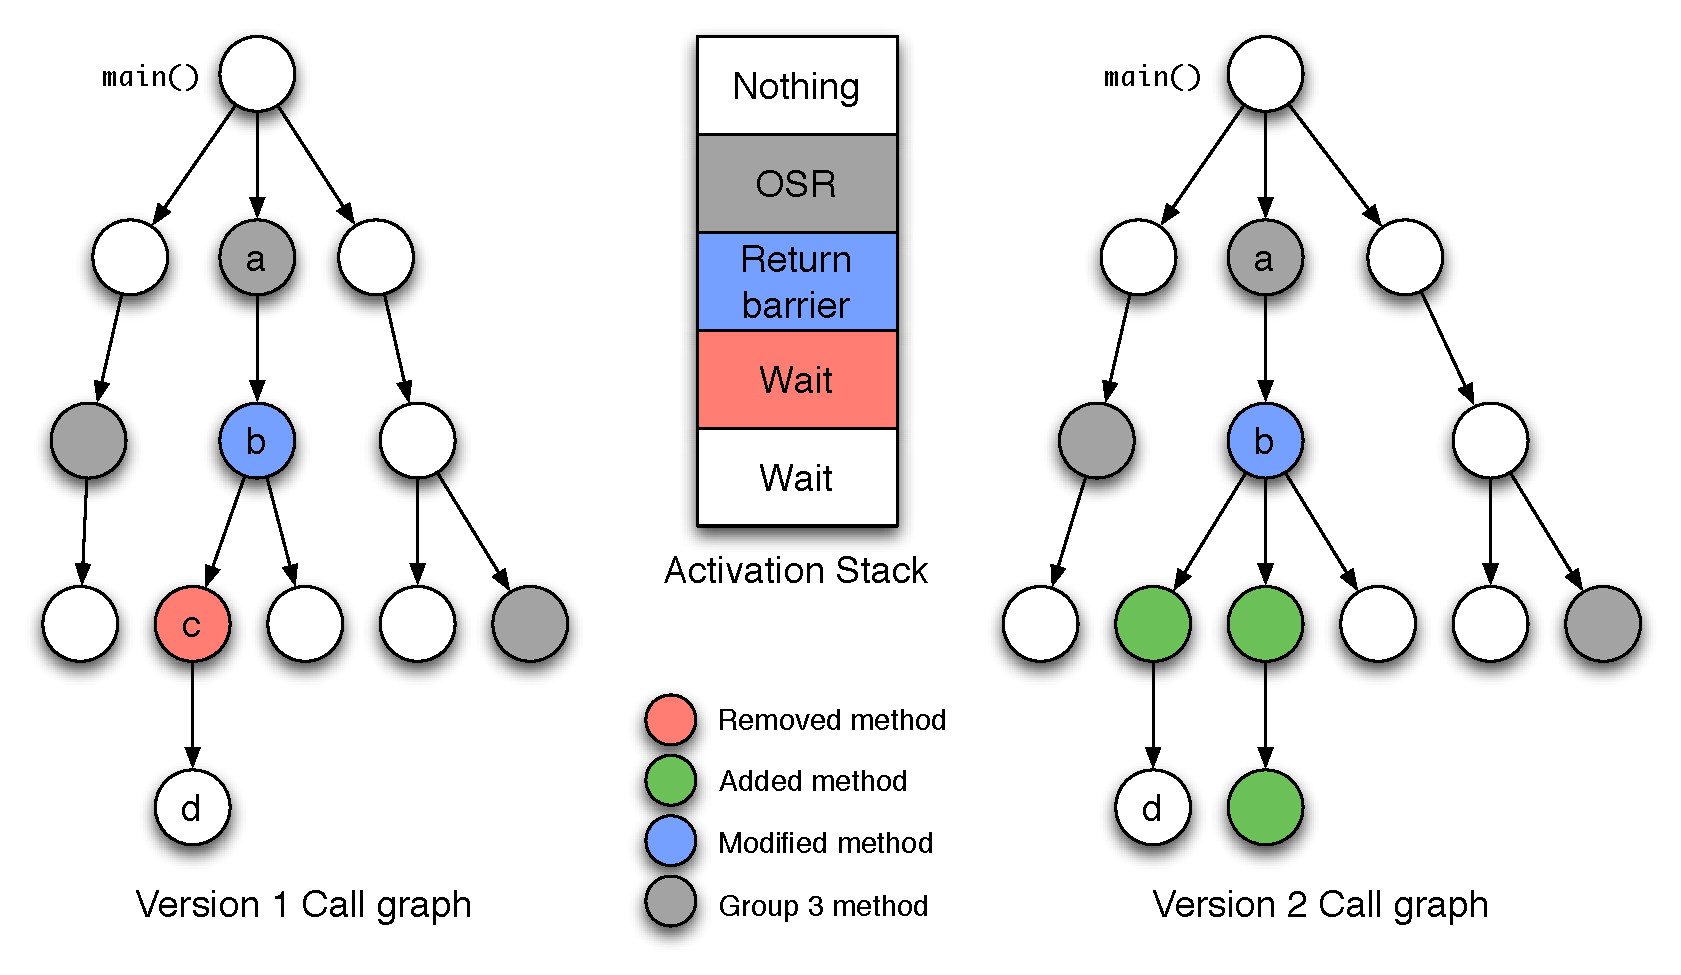
\includegraphics{images/safe-point-call-graph/both-call-graphs-3}}%
}
\end{frame}

% \begin{frame}[c,fragile]{Handling restricted methods}%{A Sub-title is optional}
% \hspace*{-5mm}
% \centering{\scalebox{0.67}{\includegraphics{images/flowchart}}}
% \end{frame}
% 
% \begin{frame}[t,fragile]{On stack replacement in \DSU{}}%{A Sub-title is optional}
% \begin{itemize}
% \item Used in \JikesRVM{} to optimize long running methods
% \item \DSU{} utilizes OSR for DSU
% \item Currently only support baseline-compiled methods
% \item Can OSR any method on stack
% \uncover<2>{
% \item Extract the state of the stack
% \item Construct a new method with a specialized prologue (at the bytecode
% level) that reconstructs the stack
% \item Last instruction of prologue jumps to bytecode where execution should
% resume from
% \item Overwrite the return address to point to the special method
% }
% \end{itemize}
% \end{frame}
% 
% 
% {
% \setbeamercovered{invisible}
% \begin{frame}[t,fragile]{OSR Example}%{A Sub-title is optional}
% \begin{footnotesize}
% \begin{columns}[t]
% 
% \begin{column}{0.4\paperwidth}
% \begin{semiverbatim}
% public class A \{
%   public int foo(int i, B b) \{
%     i = i + 1;
%     i = b.bar(i);
%     i = i + 1;
%     return i;
%   \}
% \}
% \end{semiverbatim}
% 
% \uncover<2-> {
% State: \\
% Thread: \#5 \\
% FP: 0x4ad33e40 \\
% PC: 9 \\
% Locals: i = 5, b = 0x52ae34a0 \\
% Stack vars: S0, S1, ... \\
% }
% \end{column}
% 
% \begin{column}{0.4\paperwidth}
% \begin{semiverbatim}
%  0 iload\_1
%  1 iconst\_1
%  2 iadd
%  3 istore\_1
%  4 aload\_2
%  5 iload\_1
%  6 invokevirtual <B.bar>
%  9 istore\_1
% 10 iload\_1
% 11 iconst\_1
% 12 iadd
% 13 istore\_1
% 14 iload\_1
% 15 ireturn
% \end{semiverbatim}
% \end{column}
% \end{columns}
% \end{footnotesize}
% \end{frame}
% }
% 
% {
% \setbeamercovered{invisible}
% \begin{frame}[t,fragile,shrink=20]{OSR Example}%{A Sub-title is optional}
% \begin{footnotesize}
% \begin{columns}[b]
% 
% \begin{column}{0.4\paperwidth}
% \begin{semiverbatim}
%  0 iload\_1
%  1 iconst\_1
%  2 iadd
%  3 istore\_1
%  4 aload\_2
%  5 iload\_1
%  6 invokevirtual <B.bar>
%  9 istore\_1
% 10 iload\_1
% 11 iconst\_1
% 12 iadd
% 13 istore\_1
% 14 iload\_1
% 15 ireturn
% \end{semiverbatim}
% \end{column}
% 
% \begin{column}{0.4\paperwidth}
% \begin{semiverbatim}
%    ldc 5
%    istore\_0 
%    ldc 0x52ae34a0
%    astore\_1
%    goto 9
%  0 iload\_1
%  1 iconst\_1
%  2 iadd
%  3 istore\_1
%  4 aload\_2
%  5 iload\_1
%  6 invokevirtual <B.bar>
%  9 istore\_1
% 10 iload\_1
% 11 iconst\_1
% 12 iadd
% 13 istore\_1
% 14 iload\_1
% 15 ireturn
% \end{semiverbatim}
% \end{column}
% 
% \end{columns}
% \end{footnotesize}
% \end{frame}
% }


%L  \begin{frame}[t,fragile,label=classload]{Installing new classes}%{A Sub-title is optional}
%L  \JvolveTimeLine{}{}{current}{}{}
%L  The VM maintains Class, Method and Field data structures
%L  % \begin{itemize}
%L  % \item The VM maintains Class, Method and Field data structures
%L  % \item For Method updates: Only load the new method's bytecodes
%L  % \item For Class updates: Rename the old class and load the entire class
%L  % file (equivalent to have loaded two different class)
%L  % \end{itemize}
%L  \begin{center}
%L  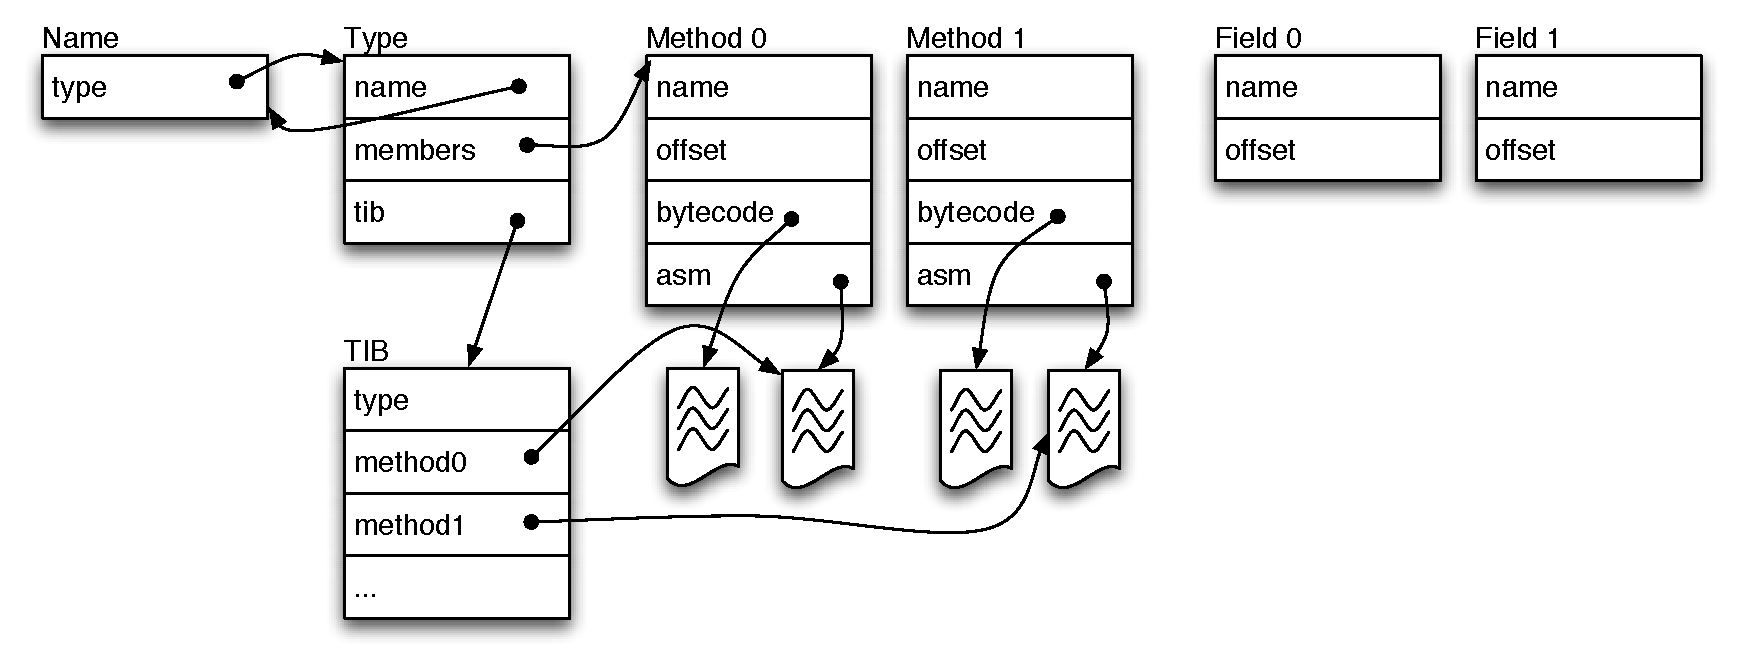
\includegraphics[scale=0.40]{images/vm-meta-data/vm-meta-data}%
%L  \end{center}
%L  \end{frame}
%L
%L  % \ifdraft{}{
%L  % {
\setbeamertemplate{headline}{}
\setbeamertemplate{footline}{}
\setbeamertemplate{navigation symbols}{}
\setbeamercovered{invisible}
\begin{frame}[t,fragile]
\vspace*{-4ex}
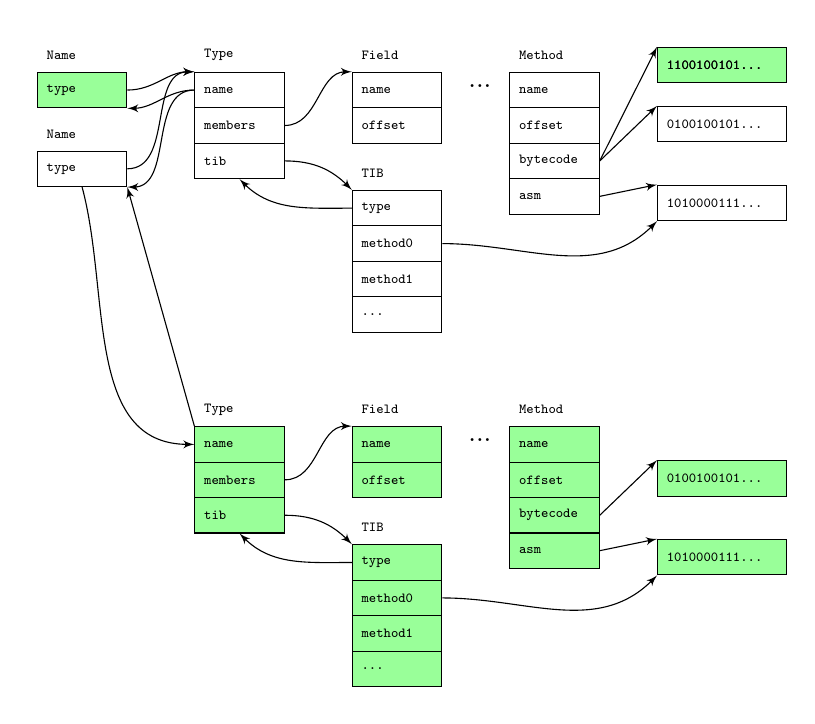
\begin{tikzpicture}[auto]

\tikzstyle{title}=[font=\tiny\tt,text width=9mm,minimum height=4.5mm]
\tikzstyle{box}=[font=\tiny\tt,draw, thin,text width=9mm,minimum height=4.5mm,anchor=north west]
% Two rows
\newcommand{\HeaderRow}[2]{% name, content
\node [title] (#1 0) { #2 }; \\
}

\newcommand{\rowsTwo}[3]{% name, row0, row1
\HeaderRow{#1}{#2}
\node [box]   (#1 1) { #3 }; \\
}
% Three rows
\newcommand{\rowsThree}[4]{% name, row0, row1, row2
\rowsTwo{#1}{#2}{#3}
\node [box]   (#1 2) { #4 }; \\
}
% Four rows
\newcommand{\rowsFour}[5]{% name, row0, row1, row2
\rowsThree{#1}{#2}{#3}{#4}
\node [box]   (#1 3) { #5 }; \\
}
% Five rows
\newcommand{\rowsFive}[6]{% name, row0, row1, row2
\rowsFour{#1}{#2}{#3}{#4}{#5}
\node [box]   (#1 4) { #6 }; \\
}

\newcommand{\newRowsTwo}[3]{% name, row0, row1
\HeaderRow{#1}{#2}
\node [box,fill=new color]   (#1 1) { #3 }; \\
}
% Three rows
\newcommand{\newRowsThree}[4]{% name, row0, row1, row2
\newRowsTwo{#1}{#2}{#3}
\node [box,fill=new color]   (#1 2) { #4 }; \\
}
% Four rows
\newcommand{\newRowsFour}[5]{% name, row0, row1, row2
\newRowsThree{#1}{#2}{#3}{#4}
\node [box,fill=new color]   (#1 3) { #5 }; \\
}
% Five rows
\newcommand{\newRowsFive}[6]{% name, row0, row1, row2
\newRowsFour{#1}{#2}{#3}{#4}{#5}
\node [box,fill=new color]   (#1 4) { #6 }; \\
}

\newcommand{\metadataTwo}[4]{% name, position, contents 
\matrix [row sep=-0.4pt,anchor=north west] (#1) at #2 {
\rowsTwo{#1}{#3}{#4}
};}
\newcommand{\metadataThree}[5]{% name, position, contents 
\matrix [row sep=-0.4pt,anchor=north west] (#1) at #2 {
\rowsThree{#1}{#3}{#4}{#5}
};}
\newcommand{\metadataFour}[6]{% name, position, contents 
\matrix [row sep=-0.4pt,anchor=north west] (#1) at #2 {
\rowsFour{#1}{#3}{#4}{#5}{#6}
};}
\newcommand{\metadataFive}[7]{% name, position, contents 
\matrix [row sep=-0.4pt,anchor=north west] (#1) at #2 {
\rowsFive{#1}{#3}{#4}{#5}{#6}{#7}
};}

\newcommand{\newMetadataTwo}[4]{% name, position, contents 
\matrix [row sep=-0.4pt,anchor=north west] (#1) at #2 {
\newRowsTwo{#1}{#3}{#4}
};}
\newcommand{\newMetadataThree}[5]{% name, position, contents 
\matrix [row sep=-0.4pt,anchor=north west] (#1) at #2 {
\newRowsThree{#1}{#3}{#4}{#5}
};}
\newcommand{\newMetadataFour}[6]{% name, position, contents 
\matrix [row sep=-0.4pt,anchor=north west] (#1) at #2 {
\newRowsFour{#1}{#3}{#4}{#5}{#6}
};}
\newcommand{\newMetadataFive}[7]{% name, position, contents 
\matrix [row sep=-0.4pt,anchor=north west] (#1) at #2 {
\newRowsFive{#1}{#3}{#4}{#5}{#6}{#7}
};}

\colorlet{new color}{green!40}
\tikzstyle{line}=[draw, thin, -latex',]
\tikzstyle{every path}=[line]

\begin{scope}
  \metadataTwo{typeref}{(0,-1)}{Name}{type}
  \uncover<4->{ \newMetadataTwo{typerefnew}{(0,0)}{Name}{type} }
  \metadataFour{class}{(2,0)}{Type}{name}{members}{tib}
  \metadataThree{field}{(4,0)}{Field}{name}{offset}
  \node at (5.75,-0.75) {...};
  \metadataFive{method}{(6,0)}{Method}{name}{offset}{bytecode}{asm}
  \metadataFive{tib}{(4,-1.5)}{TIB}{type}{method0}{method1}{...}
  \uncover<-2>{ \node[box,text width=14mm] (bc) at (8,-1)   { 0100100101...  }; }
  \node[box,text width=14mm] (mc) at (8,-2)   { 1010000111... };
  \uncover<2> { \node[box,text width=14mm,fill=new color] (bcnew) at (8,-0.25) { 1100100101... }; }
  \uncover<3->{ \node[box,text width=14mm] (bcnew) at (8,-0.25) { 1100100101... }; }
\end{scope}

\uncover<-3> { \path (typeref 1.east) to [out=0,in=180] (class 1.north west); }
\uncover<-3> { \path (class 1.west)   to [out=180,in=0] (typeref 1.south east); }
\uncover<4-> { \path (typerefnew 1.east) to [out=0,in=180] (class 1.north west); }
\uncover<4-> { \path (class 1.west)   to [out=180,in=0] (typerefnew 1.south east); }
\path (class 2.east)         to [out=0,in=180]   (field 1.north west);
\path (class 3.east)         to [out=0,in=135]   (tib 1.north west);
\path (tib 1.west)           to [out=180,in=315] (class 3.south);
\path (tib 2.east)           to [out=0,in=225]   (mc.south west);
\path (method 4.east)        to                  (mc.north west);
\uncover<1>  { \path (method 3.east)        to   (bc.north west);    }
\uncover<2-> { \path (method 3.east)        to   (bcnew.north west); }

\uncover<5->{
\begin{scope}[yshift=-4.5cm]
  \newMetadataFour{class1}{(2,0)}{Type}{name}{members}{tib}
  \newMetadataThree{field1}{(4,0)}{Field}{name}{offset}
  \node at (5.75,-0.75) {...};
  \newMetadataFive{method1}{(6,0)}{Method}{name}{offset}{bytecode}{asm}
  \newMetadataFive{tib1}{(4,-1.5)}{TIB}{type}{method0}{method1}{...}
  \node[box,text width=14mm,fill=new color] (bc1) at (8,-1) { 0100100101... };
  \node[box,text width=14mm,fill=new color] (mc1) at (8,-2) { 1010000111... };
\end{scope}
  \path (class1 2.east)         to [out=0,in=180]   (field1 1.north west);
  \path (class1 3.east)         to [out=0,in=135]   (tib1 1.north west);
  \path (tib1 2.east)           to [out=0,in=225]   (mc1.south west);
  \path (tib1 1.west)           to [out=180,in=315] (class1 3.south);
  \path (method1 3.east)        to                  (bc1.north west);
  \path (method1 4.east)        to                  (mc1.north west);
  \path (class1 1.north west)   to                  (typeref 1.south east);
  \path (typeref 1.south)       to [out=285,in=180] (class1 1.west);
}

\end{tikzpicture}
\end{frame}
}

%L  % }
%L
%L  \begin{frame}{Updating a method}%{A Sub-title is optional}
%L  \vspace*{-1mm}%
%L  \begin{center}
%L  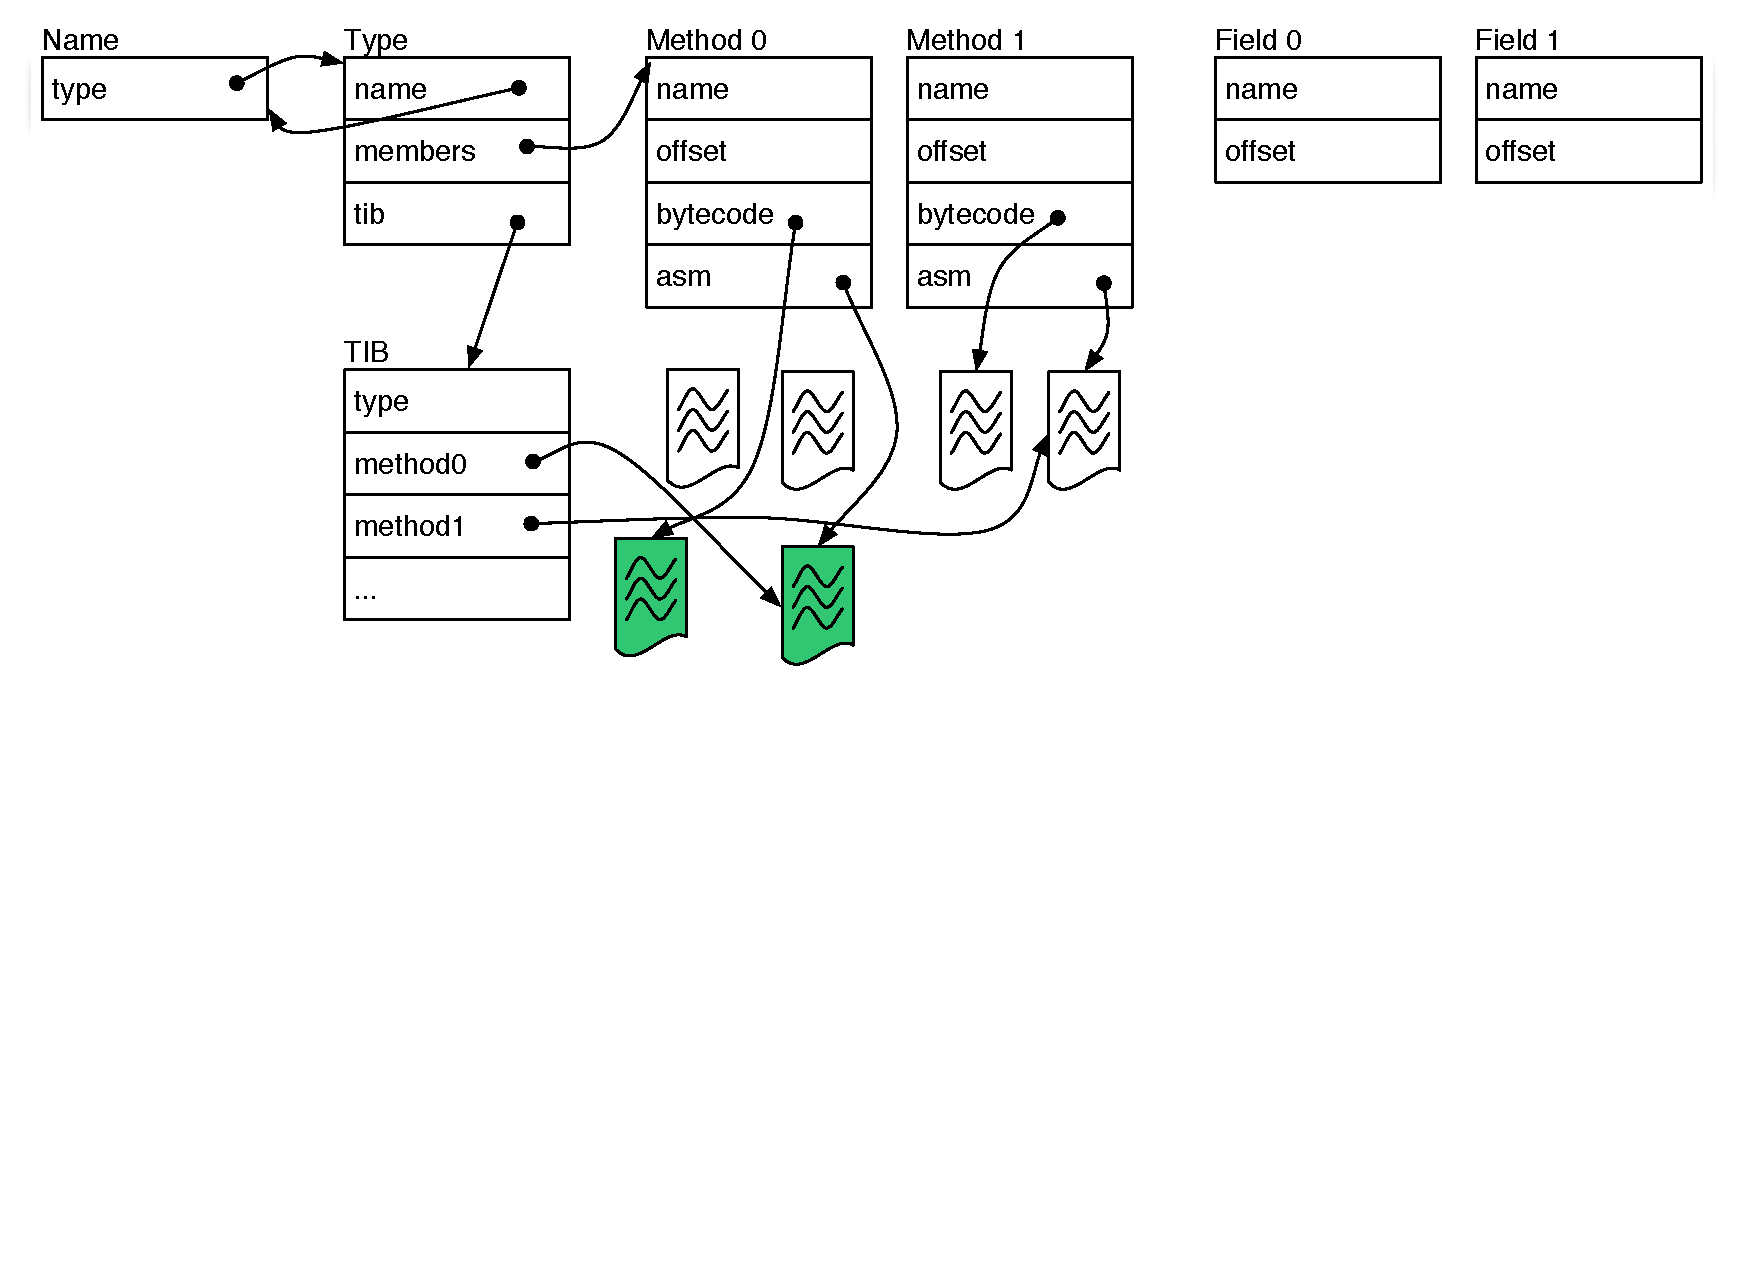
\includegraphics[scale=0.36]{images/vm-meta-data/vm-meta-data-updated-method}%
%L  \end{center}
%L  \end{frame}
%L
%L  \begin{frame}{Updating a class}%{A Sub-title is optional}
%L  \vspace*{-1mm}%
%L  \begin{center}
%L  \includegraphics[scale=0.36]<1>{images/vm-meta-data/vm-meta-data-renamed-class}%
%L  \includegraphics[scale=0.36]<2>{images/vm-meta-data/vm-meta-data-updated-class}%
%L  \end{center}
%L  \end{frame}

\begin{frame}{Update code}%{A Sub-title is optional}
\vspace*{-3mm}%
\begin{center}%
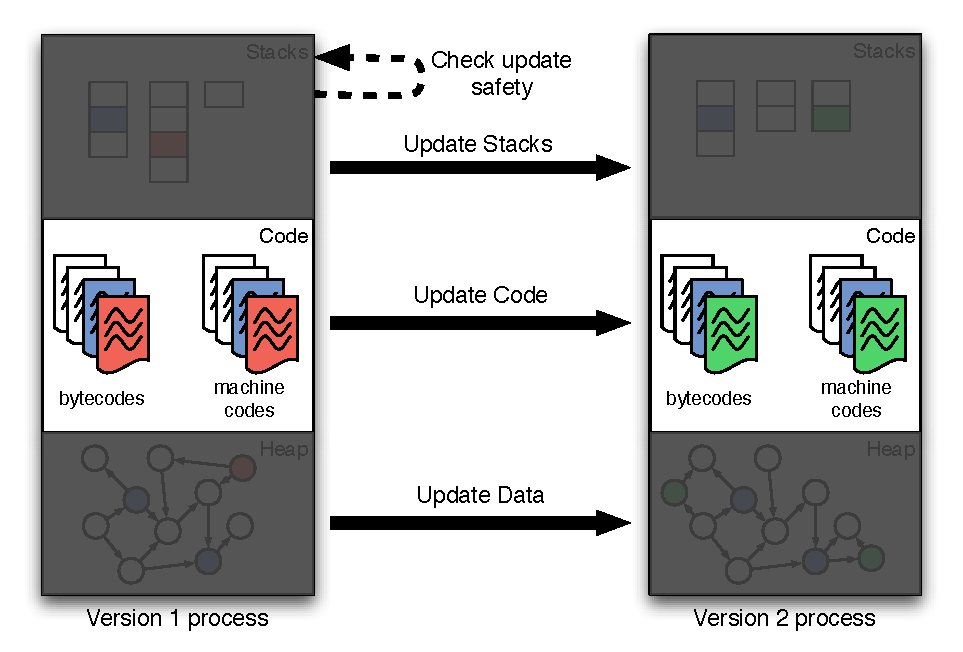
\includegraphics[scale=0.73]{images/process-state/both-process-state-highlight-code}%
\end{center}%
\end{frame}

\begin{frame}{Update code}%{A Sub-title is optional}
\begin{itemize}
\item Modify class loader to recognize new versions of classes
\item Install new versions of classes and methods
\item Rely on Just-in-time Compiler to compile new versions of methods on
demand
\item Extend On-stack replacement to update active methods
\end{itemize}
\end{frame}

% \begin{frame}{Updating a method}%{A Sub-title is optional}
% \vspace*{-1mm}%
% \begin{center}
% 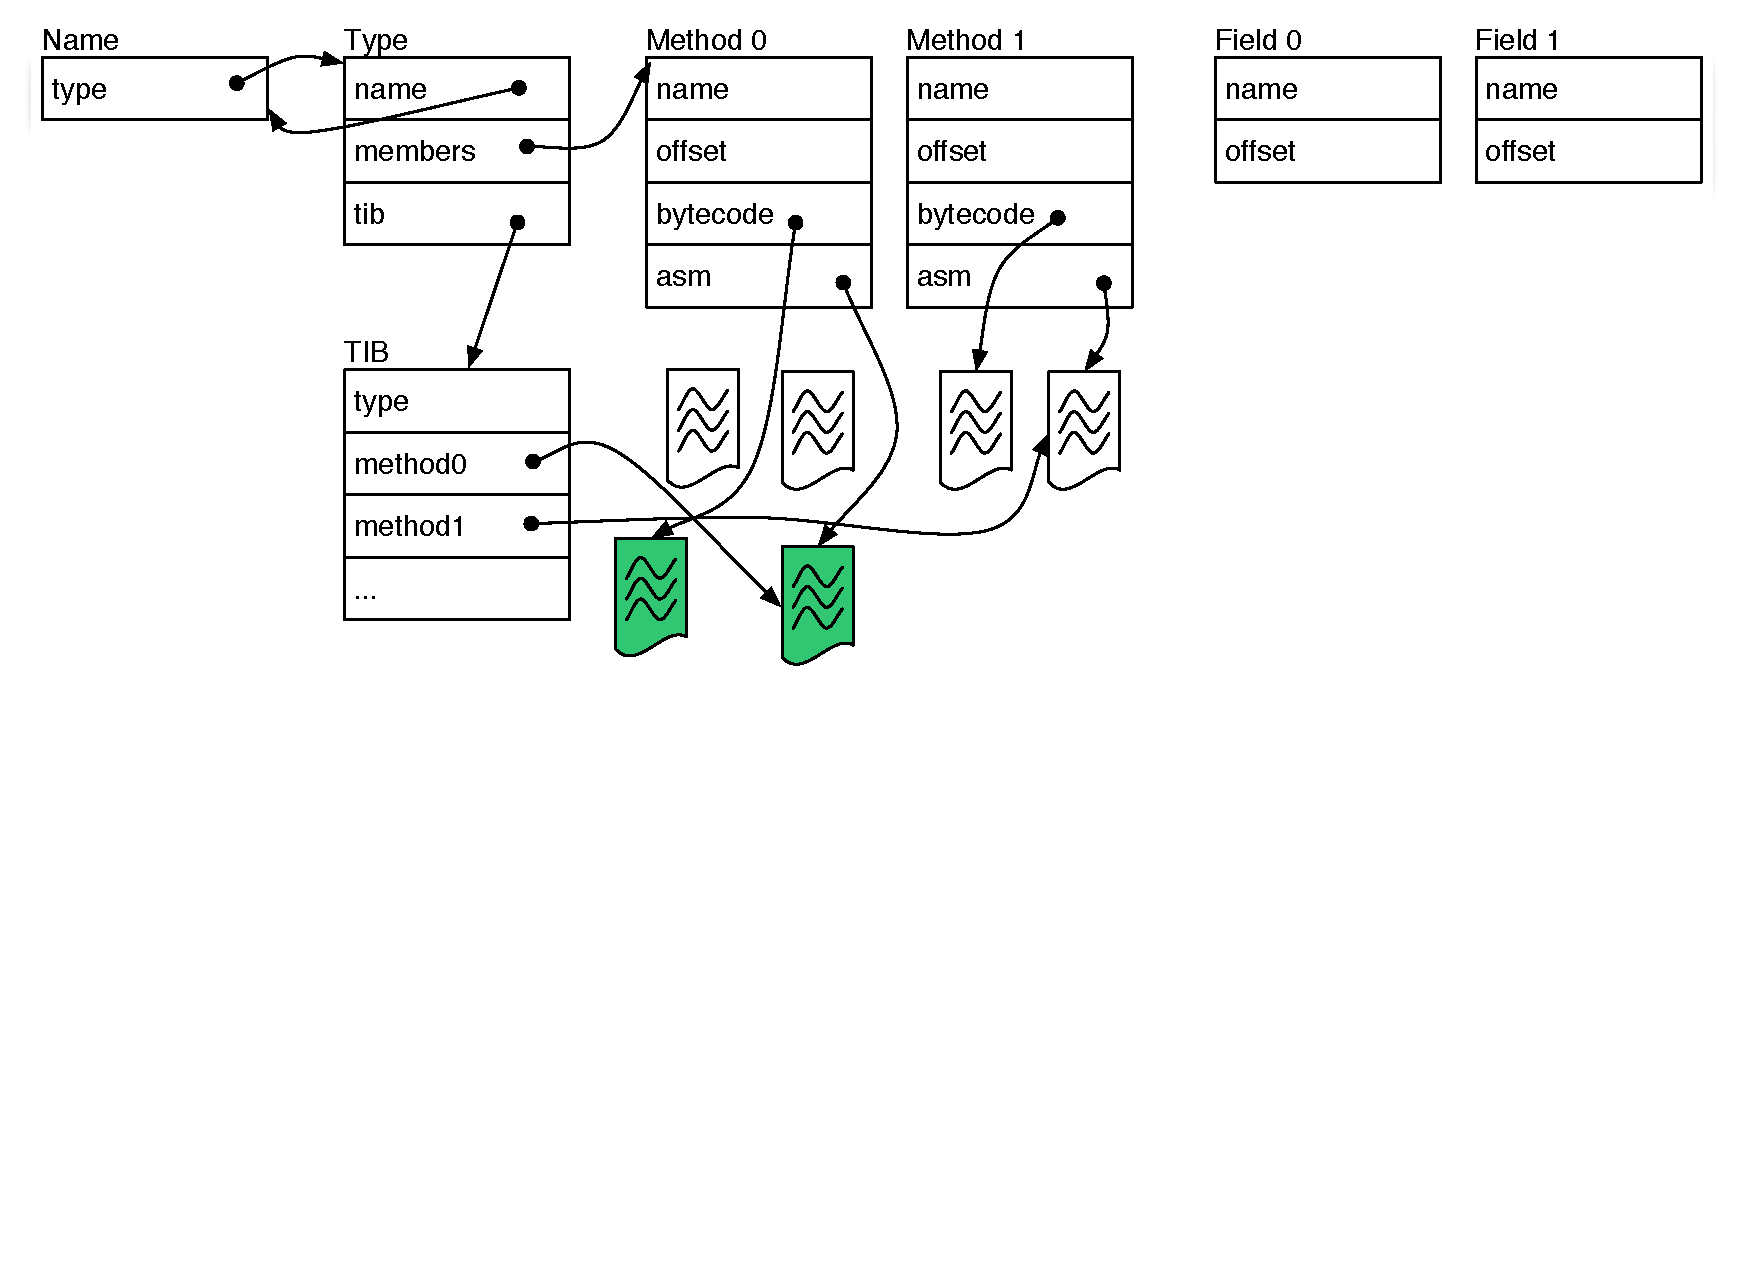
\includegraphics[scale=0.36]{images/vm-meta-data/vm-meta-data-updated-method}%
% \end{center}
% \end{frame}
% 
% \begin{frame}{Updating a class}%{A Sub-title is optional}
% \vspace*{-1mm}%
% \begin{center}
% \only<1>{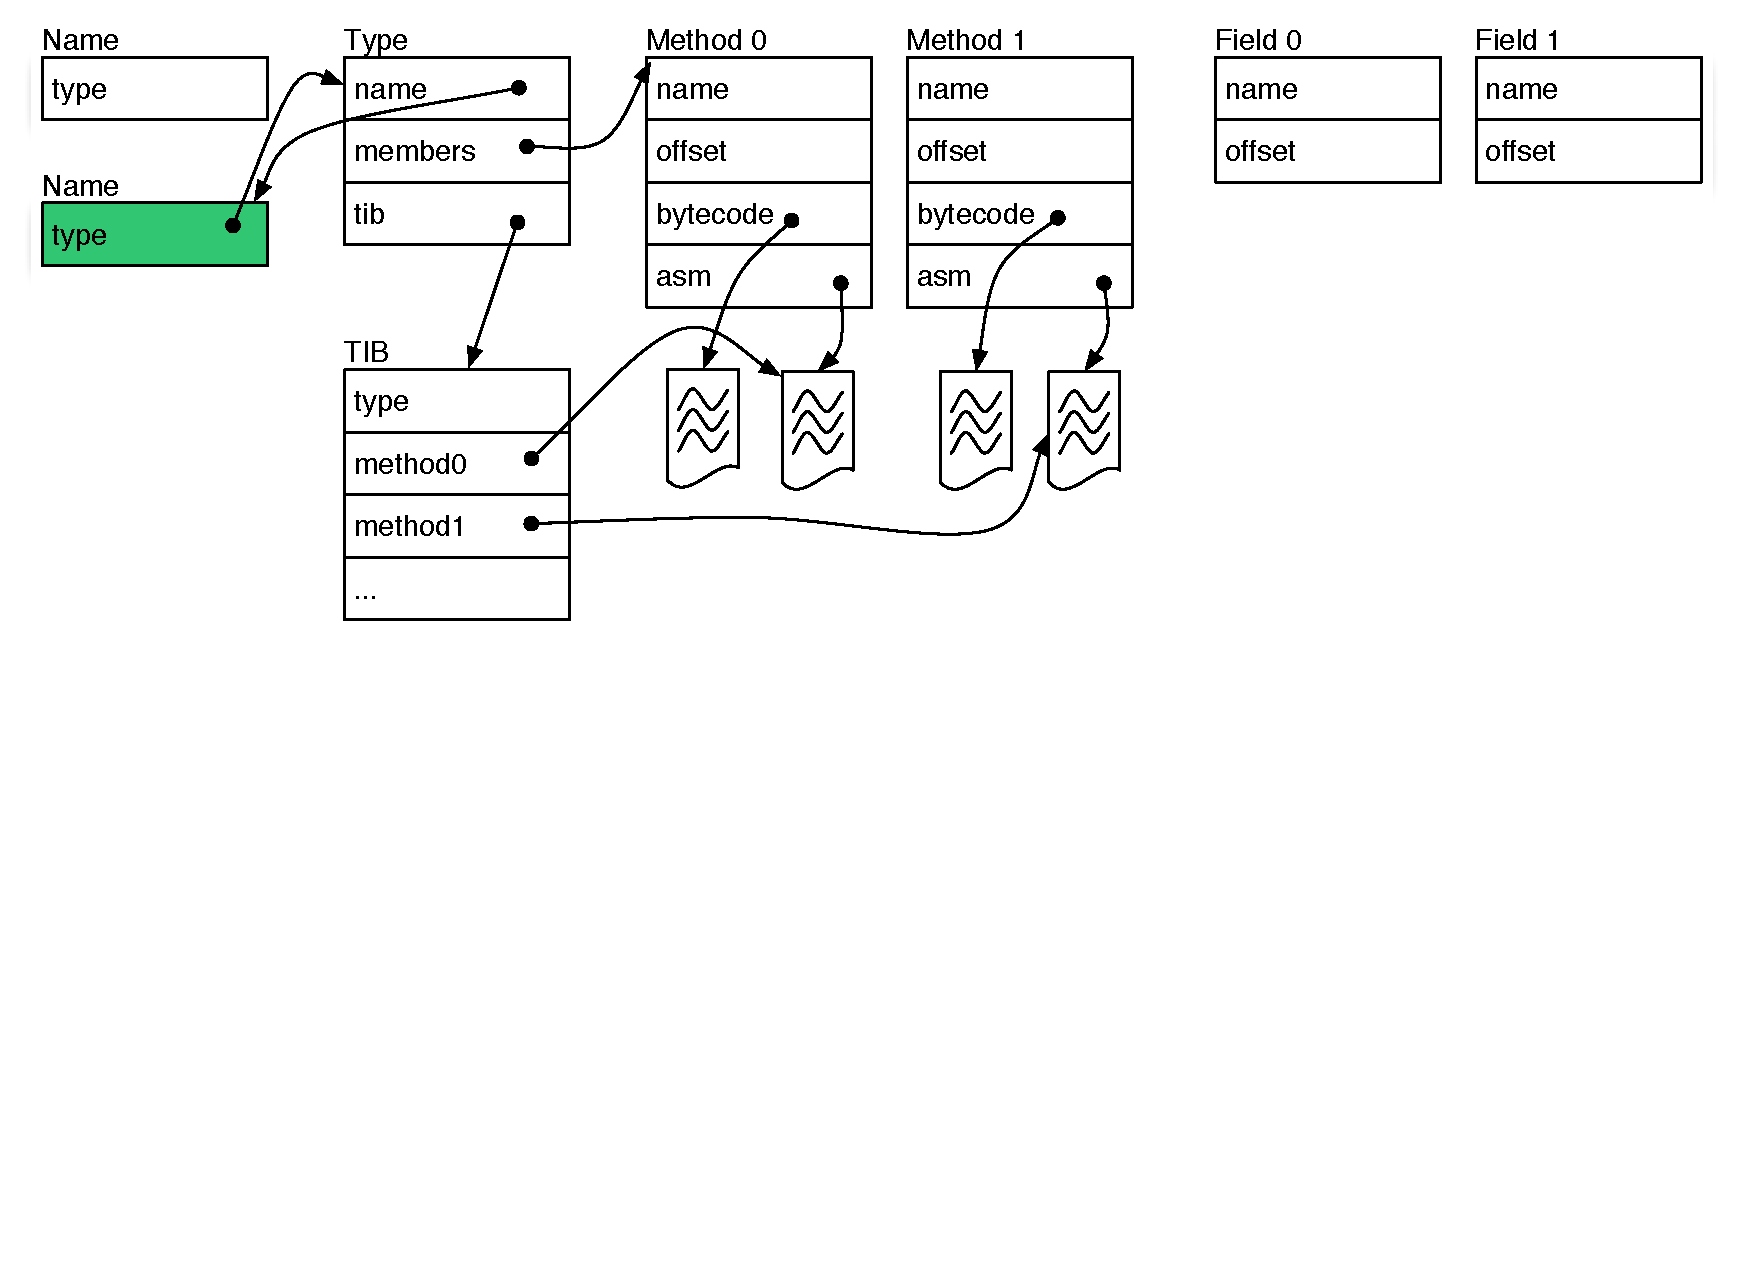
\includegraphics[scale=0.36]{images/vm-meta-data/vm-meta-data-renamed-class}}%
% \only<2>{\includegraphics[scale=0.36]{images/vm-meta-data/vm-meta-data-updated-class}}%
% \end{center}
% \end{frame}

\begin{frame}{Update data}%{A Sub-title is optional}
\vspace*{-3mm}%
\begin{center}%
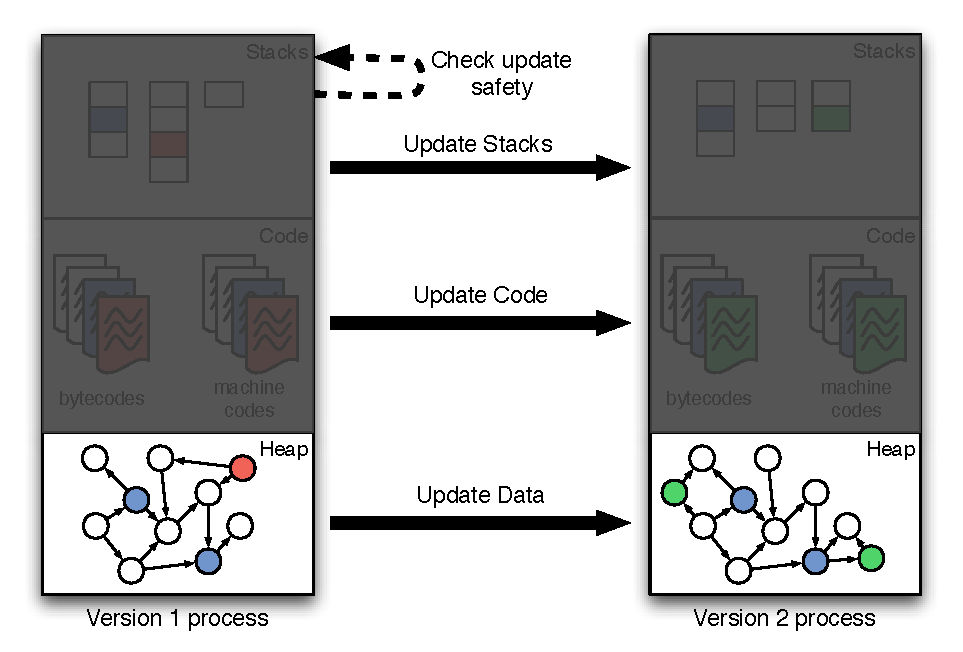
\includegraphics[scale=0.73]{images/process-state/both-process-state-highlight-heap}%
\end{center}%
\end{frame}

% \newcommand{\ExampleCodeSize}{footnotesize}

% \newcommand{\removed}[1]{\textcolor{red}{- #1}}
% \newcommand{\addedxx}[1]{\textcolor{OliveGreen}{+ #1}}

\begin{frame}[fragile,shrink=5]{Example of an update (JavaEmailServer)}%{A Sub-title is optional}
\begin{\ExampleCodeSize}
\begin{semiverbatim}
  public class User \{
    private final String username, domain, password;
\removed{  private String[] forwardAddresses;}
\addedxx{  private EmailAddress[] forwardAddresses;}
    public User(...) \{...\}
    public String[] getForwardedAddresses() \{...\}

    public void setForwardedAddresses(String[] f) \{...\}

  \}

  public class ConfigurationManager \{
    private User loadUser(...) \{
       ...
       User user = new User(...);
       String[] f = ...;

       user.setForwardedAddresses(f);
       return user;
    \}
  \}
\end{semiverbatim}
\end{\ExampleCodeSize}
\end{frame}


% \begin{frame}[fragile,shrink=5]{Example of an update (JavaEmailServer)}%{A Sub-title is optional}
% \begin{\ExampleCodeSize}
% \begin{semiverbatim}
% public class User \{
%   private String username, domain, password;
%   private \sout{String[]} EmailAddress[] forwardAddresses;
%   public \sout{String[]} EmailAddress[] getForwardedAddresses() \{...\}
%   public void setForwardedAddresses(\sout{String[]} EmailAddress[] f) \{...\}
% \}
% 
% public class ConfigurationManager \{
%   private User loadUser(...) \{
%      ...
%      User user = new User(...);
%      \sout{String[]} EmailAddress[] f = ...;
%      user.setForwardedAddresses(f);
%      return user;
%   \}
% \}
% 
% \end{semiverbatim}
% \end{\ExampleCodeSize}
% \end{frame}

\begin{frame}[fragile,shrink=5]{Example of an update (JavaEmailServer)}%{A Sub-title is optional}
\begin{\ExampleCodeSize}
\begin{semiverbatim}
  public class User \{
    private final String username, domain, password;
\removed{  private String[] forwardAddresses;}
\addedxx{  private EmailAddress[] forwardAddresses;}
    public User(...) \{...\}
\removed{  public String[] getForwardedAddresses() \{...\}}
\addedxx{  public EmailAddress[] getForwardedAddresses() \{...\}}
\removed{  public void setForwardedAddresses(String[] f) \{...\}}
\addedxx{  public void setForwardedAddresses(EmailAddress[] f) \{...\}}
  \}

  public class ConfigurationManager \{
    private User loadUser(...) \{
       ...
       User user = new User(...);
\removed{     String[] f = ...;}
\addedxx{     EmailAddress[] f = ...;}
       user.setForwardedAddresses(f);
       return user;
    \}
  \}
\end{semiverbatim}
\end{\ExampleCodeSize}
\end{frame}

\begin{frame}[fragile,shrink=5]{Example of an update (JavaEmailServer)}%{A Sub-title is optional}
\mode<beamer> {
\begin{textblock*}{46mm}[0,0](79mm,20mm)
\begin{block}{}
Stub generated by UPT for the old version
\end{block}
\end{textblock*}
\only<1>{
\begin{textblock*}{46mm}[0,0](79mm,48mm)
\begin{block}{}
Default transformer copies old fields, initializes new ones to
\texttt{null}
\end{block}
\end{textblock*}}
}
\begin{small}
\begin{semiverbatim}
public class v131_User \{
  private final String username, domain, password;
  private String[] forwardAddresses;
\}
public class JvolveTransformers \{
 ...
 public static void jvolveClass(User unused) \{\}
 public static void jvolveObject(User to, v131_User from) \{
    to.username = from.username;
    to.domain = from.domain;
    to.password = from.password;
    // to.forwardAddresses = null;
    \uncover<2>{int len = from.forwardAddresses.length;
    to.forwardAddresses = new EmailAddress[len];
    for (int i = 0; i < len; i++) \{
      to.forwardAddresses[i] =
        new EmailAddress(from.forwardAddresses[i]);
}\}\}\}

\end{semiverbatim}
\end{small}
\end{frame}



\begin{frame}[t]{Transforming objects in the GC}%{A Sub-title is optional}
\vspace*{-6ex}
\begin{center}
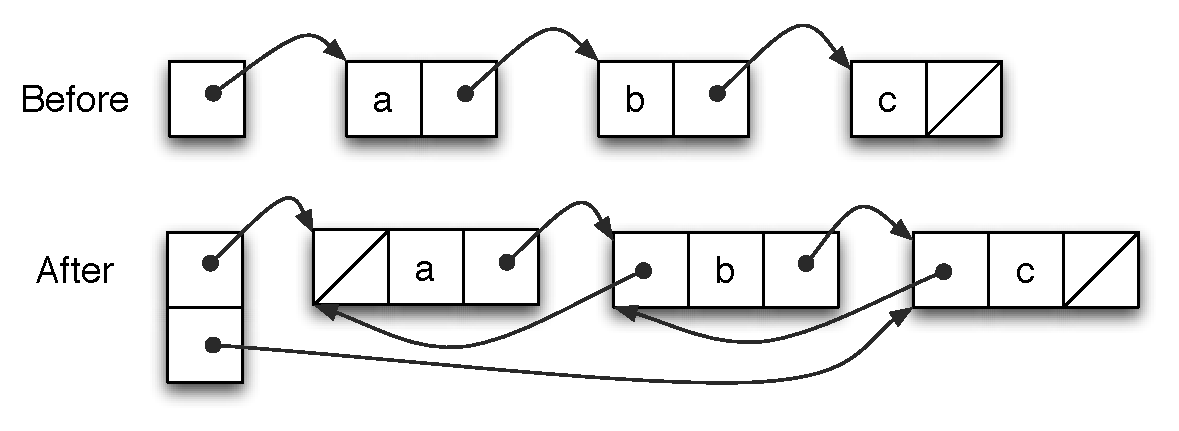
\includegraphics[scale=0.6]{images/singly-doubly/linked-lists-without-gc}%
\end{center}
Happens in two steps \\
\begin{itemize}
\item Garbage collector creates an additional empty copy for updated objects
\item Walk through and transform all these objects
\end{itemize}
% \begin{itemize}
% % \item Supported on top of a semi-space copying collector
% % \item Regular GC
% %   \begin{itemize}
% %   \item Copies all live objects to ``to'' space
% %   \end{itemize}
% \item Jvolve's GC
%   \begin{itemize}
%   \item Built on top of a semi-space copying collector
%   \item Copies all live objects to ``to'' space
%   \item For updated objects, allocate an empty object in ``to'' space
%   \item Forwarding pointers and object pointers point to these empty
%   objects
%   \item After GC, walk through all updated objects and run their
%   transformation functions
%   \end{itemize}
% \end{itemize}
\end{frame}

% \ifdraft{}{
% 
%%%%%%%%%%%%%%%%%%%%%%%%%%%%%%%%%%%%%%%%%%%%%%%%%%%%%%%%%%%%%%%%%%%%%%%%
% Colors
\colorlet{black object color}{black!60}
\colorlet{grey object color}{black!20}
\colorlet{forwarding pointer color}{structure.fg!40}
\colorlet{dsu v0 color}{blue!60}
\colorlet{dsu v1 empty color}{blue!20}
\colorlet{dsu forwarding pointer color}{forwarding pointer color!50!dsu v0 color}
%%%%%%%%%%%%%%%%%%%%%%%%%%%%%%%%%%%%%%%%%%%%%%%%%%%%%%%%%%%%%%%%%%%%%%%%

%%%%%%%%%%%%%%%%%%%%%%%%%%%%%%%%%%%%%%%%%%%%%%%%%%%%%%%%%%%%%%%%%%%%%%%%
% Define the style for each field of the object
\newlength{\drawthickness}
\setlength{\drawthickness}{0.6pt}
\newlength{\fielddimension}
\setlength{\fielddimension}{5mm}
\tikzstyle{field}=[
    rectangle,
    draw=black,
    line width=\drawthickness,
    minimum width=\fielddimension,
    minimum height=\fielddimension,
    inner sep=0pt,
    font=\tiny,
]
\tikzstyle{new space grey field}=[field,fill=grey object color]
\tikzstyle{new space black field}=[field,fill=black object color]
\tikzstyle{dsu v0 field}=[field,fill=dsu v0 color]
\tikzstyle{dsu v1 empty field}=[field,fill=dsu v1 empty color]
%%%%%%%%%%%%%%%%%%%%%%%%%%%%%%%%%%%%%%%%%%%%%%%%%%%%%%%%%%%%%%%%%%%%%%%%

%%%%%%%%%%%%%%%%%%%%%%%%%%%%%%%%%%%%%%%%%%%%%%%%%%%%%%%%%%%%%%%%%%%%%%%%
% Define the style for each object
\tikzstyle{object}=[
    column sep=-\drawthickness,
    nodes=field,
    inner sep=0pt,
]
\tikzstyle{new space grey object}=[object,nodes=new space grey field]
\tikzstyle{new space black object}=[object,nodes=new space black field]
\tikzstyle{dsu v0 object}=[object,nodes=dsu v0 field]
\tikzstyle{dsu v1 empty object}=[object,nodes=dsu v1 empty field]
%%%%%%%%%%%%%%%%%%%%%%%%%%%%%%%%%%%%%%%%%%%%%%%%%%%%%%%%%%%%%%%%%%%%%%%%

%%%%%%%%%%%%%%%%%%%%%%%%%%%%%%%%%%%%%%%%%%%%%%%%%%%%%%%%%%%%%%%%%%%%%%%%
% Style for arrows
\tikzstyle{regular}=[-to,draw]
\tikzstyle{transparent}=[-to,draw=black!15!bg]
%%%%%%%%%%%%%%%%%%%%%%%%%%%%%%%%%%%%%%%%%%%%%%%%%%%%%%%%%%%%%%%%%%%%%%%%

%%%%%%%%%%%%%%%%%%%%%%%%%%%%%%%%%%%%%%%%%%%%%%%%%%%%%%%%%%%%%%%%%%%%%%%%
% Define a macro for creating an object with two fields
\newcommand{\twoFieldsObject}[3]{% name, position, object style
\matrix[#3,ampersand replacement=\&] (#1) at #2 {
  \node (#1 0) {}; \& \node (#1 1) {}; \\
};}
\newcommand{\fourFieldsObject}[3]{% name, position, object style
\matrix[#3,ampersand replacement=\&] (#1) at #2 {
  \node (#1 0) {}; \& \node (#1 1) {}; \& \node (#1 2) {}; \& \node (#1 3) {}; \\
};}


% Command to write a label next to an object
\newcommand{\labelObject}[4]{% label text, object name, label position, label anchor
\draw (#2.#3) node[anchor=#4,inner sep=0.5pt,font=\tiny] {#1};}
\newcommand{\oldSpaceLabelObject}[2]{% label text, object name
\labelObject{#1}{#2}{north west}{north east}}
\newcommand{\newSpaceLabelObject}[2]{% label text, object name
\labelObject{#1}{#2}{150}{south west}}

\newcommand{\oldSpaceObject}[3][object]{% object style, name, position
\twoFieldsObject{#2}{#3}{#1}\oldSpaceLabelObject{#2}{#2}}
\newcommand{\dsuOldSpaceVersionZeroObject}[2]{% name, location
\twoFieldsObject{#1}{#2}{dsu v0 object}\oldSpaceLabelObject{#1 $v_0$}{#1}}
\newcommand{\dsuOldSpaceVersionOneObject}[2]{% name, location
\fourFieldsObject{#1 v1}{#2}{dsu v1 empty object}\oldSpaceLabelObject{#1 $v_1$}{#1 v1}}

\newcommand{\newSpaceObject}[4][]{% extra name, name, position, object style
\twoFieldsObject{#2}{#3}{#4}\newSpaceLabelObject{#2#1}{#2}}
\newcommand{\newSpaceVersionOneEmptyObject}[2]{% name, position
\fourFieldsObject{#1 v1}{#2}{dsu v1 empty object}\labelObject{#1 $v_1$}{#1 v1}{165}{south west}}
\newcommand{\newSpaceGreyObject}[2]{% name, position
\newSpaceObject{#1}{#2}{new space grey object}}
\newcommand{\newSpaceBlackObject}[2]{% name, position
\newSpaceObject{#1}{#2}{new space black object}}
\newcommand{\dsuNewSpaceGreyObject}[2]{% name, position
\newSpaceObject[\ $v_0$]{#1}{#2}{new space grey object}}
\newcommand{\dsuNewSpaceBlackObject}[2]{% name, position
\newSpaceObject[\ $v_0$]{#1}{#2}{new space black object}}

\newcommand{\forwardingPointer}[1]{% name
\node[field,minimum width=2\fielddimension,fill=forwarding pointer color] at (#1.center) {#1'};
}
\newcommand{\dsuForwardingPointer}[1]{% name
\node[field,minimum width=2\fielddimension,fill=dsu forwarding pointer color] at (#1.center) {#1' $v_1$};
}
%%%%%%%%%%%%%%%%%%%%%%%%%%%%%%%%%%%%%%%%%%%%%%%%%%%%%%%%%%%%%%%%%%%%%%%%

%%%%%%%%%%%%%%%%%%%%%%%%%%%%%%%%%%%%%%%%%%%%%%%%%%%%%%%%%%%%%%%%%%%%%%%%
% Define coordinates of the various objects
\newcommand{\objectRoot}{(-3,0.8)}
\newcommand{\objectA}{(0,0)}
\newcommand{\objectB}{(-2,-1)}
\newcommand{\objectC}{(2,-1)}
\newcommand{\objectD}{(-3,-2)}
\newcommand{\objectE}{(-1,-2)}
\newcommand{\objectF}{(1,-2)}
\newcommand{\objectG}{(3,-2)}

\newcommand{\objectAprime}{(-3.5,0.25)}
\newcommand{\objectBprime}{(-2.5,0.25)}
\newcommand{\objectCprime}{(-1.5,0.25)}
\newcommand{\objectDprime}{(-0.5,0.25)}
\newcommand{\objectEprime}{(+0.5,0.25)}
\newcommand{\objectFprime}{(+1.5,0.25)}
\newcommand{\objectGprime}{(+2.5,0.25)}

% old space
\newcommand{\objectCVersionOne}{(2.5,0)}
\newcommand{\objectFVersionOne}{(1,-3)}
% new space
\newcommand{\objectCprimeVersionOne}{(-3,-1.75)}
\newcommand{\objectFprimeVersionOne}{(-0.75,-1.75)}
%%%%%%%%%%%%%%%%%%%%%%%%%%%%%%%%%%%%%%%%%%%%%%%%%%%%%%%%%%%%%%%%%%%%%%%%

% vim:tw=0:nospell

% % 
% The various steps of the animation are
% Slide 1: Show all objects
% Slide 2: A is copied
% Slide 3: A is scanned; B, C are copied
% Slide 4: A, B are scanned; C, D, E are copied
% Slide 5: A, B, C are scanned; D, E, F, G are copied
% Slide 6: A-D are scanned
% Slide 7: A-E are scanned
% Slide 8: A-F are scanned
% Slide 9: A-G are scanned
{
\begin{frame}[fragile]{Semi-space copying collector}%{A Sub-title is optional}
\setbeamercovered{invisible}
\begin{columns}[t]
\begin{column}[T]{0.67\paperwidth}
\begin{tikzpicture}
\begin{scope}
  % objects
  \uncover<1>{       \node[field] (root) at \objectRoot {root};                        }
  \uncover<2->{      \node[new space black field] (root) at \objectRoot {root};        }
                     \oldSpaceObject{A}{\objectA}
                     \oldSpaceObject{B}{\objectB}
                     \oldSpaceObject{C}{\objectC}
                     \oldSpaceObject{D}{\objectD}
                     \oldSpaceObject{E}{\objectE}
                     \oldSpaceObject{F}{\objectF}
                     \oldSpaceObject{G}{\objectG}
  % forwarding pointers
  \uncover<2->{      \forwardingPointer{A}                             }
  \uncover<3->{      \forwardingPointer{B}
                     \forwardingPointer{C}                             }
  \uncover<4->{      \forwardingPointer{D}
                     \forwardingPointer{E}                             }
  \uncover<5->{      \forwardingPointer{F}
                     \forwardingPointer{G}                             }
  % pointer arrows
  \uncover<1>   {    \path[regular]     (root.east)  to [out=330,in=120] (A.140)    ;          }
  \uncover<1>   {    \path[regular]     (A 0.center) to                (B.90)     ;            }
  \uncover<1>   {    \path[regular]     (A 1.center) to                (C.135)    ;            }
  \uncover<1-2> {    \path[regular]     (B 0.center) to                (D.135)    ;            }
  \uncover<1-2> {    \path[regular]     (B 1.center) to                (E.90)     ;            }
  \uncover<1-2> {    \path[regular]     (C 0.center) to                (F.135)    ;            }
  \uncover<1-2> {    \path[regular]     (C 1.center) to                (G.90)     ;            }
  \uncover<1-4> {    \path[regular]     (F 0.center) to                (A)        ;            }
                                                                      
  \uncover<2> {    \path[transparent]   (root.east)  to [out=0,in=120] (A.140)    ;            }
  \uncover<2> {    \path[transparent]   (A 0.center) to                (B.90)     ;            }
  \uncover<2> {    \path[transparent]   (A 1.center) to                (C.135)    ;            }
  \uncover<3> {    \path[transparent]   (B 0.center) to                (D.135)    ;            }
  \uncover<3> {    \path[transparent]   (B 1.center) to                (E.90)     ;            }
  \uncover<3> {    \path[transparent]   (C 0.center) to                (F.135)    ;            }
  \uncover<3> {    \path[transparent]   (C 1.center) to                (G.90)     ;            }
  \uncover<5> {    \path[transparent]   (F 0.center) to                (A)        ;            }

  \draw[draw,thin] (-4,-2.5) rectangle (4,0.5);
  \draw (4,0.5) node[anchor=north east,inner sep=1pt,font=\tiny] {FromSpace};

\end{scope}
\begin{scope}[yshift=-3.75cm]
  % objects
  \uncover<2>   {    \newSpaceGreyObject{A'}{\objectAprime}                          }
  \uncover<3->  {    \newSpaceBlackObject{A'}{\objectAprime}                         }

  \uncover<3>   {    \newSpaceGreyObject{B'}{\objectBprime}                          }
  \uncover<4->  {    \newSpaceBlackObject{B'}{\objectBprime}                         }

  \uncover<3-4> {    \newSpaceGreyObject{C'}{\objectCprime}                          }
  \uncover<5->  {    \newSpaceBlackObject{C'}{\objectCprime}                         }

  \uncover<4-5> {    \newSpaceGreyObject{D'}{\objectDprime}                          }
  \uncover<6->  {    \newSpaceBlackObject{D'}{\objectDprime}                         }

  \uncover<4-6> {    \newSpaceGreyObject{E'}{\objectEprime}                          }
  \uncover<7->  {    \newSpaceBlackObject{E'}{\objectEprime}                         }

  \uncover<5-7> {    \newSpaceGreyObject{F'}{\objectFprime}                          }
  \uncover<8->  {    \newSpaceBlackObject{F'}{\objectFprime}                         }

  \uncover<5-8> {    \newSpaceGreyObject{G'}{\objectGprime}                          }
  \uncover<9->  {    \newSpaceBlackObject{G'}{\objectGprime}                         }

  % pointer arrows
  \uncover<2->  {    \path[regular] (root.west)   to [out=220,in=95] (A'.north west);    }
  \uncover<2>   {    \path[regular] (A' 0.center) to [out=130,in=180] (B.west);
                     \path[regular] (A' 1.center) to [out=70,in=180]  (C.west);           }
  \uncover<3->  {    \path[regular] (A' 0.center) to [out=80,in=135]  (B'.150);          
                     \path[regular] (A' 1.center) to [out=70,in=150]  (C'.150);           }
                                                                                         
  \uncover<3>   {    \path[regular] (B' 0.center) to                  (D.south);         
                     \path[regular] (B' 1.center) to                  (E.south);          }
  \uncover<4->  {    \path[regular] (B' 0.center) to [out=300,in=240] (D'.215);          
                     \path[regular] (B' 1.center) to [out=330,in=240] (E'.215);           }
                                                                                         
  \uncover<3-4> {    \path[regular] (C' 0.center) to                  (F.south);         
                     \path[regular] (C' 1.center) to                  (G.south west);     }
  \uncover<5->  {    \path[regular] (C' 0.center) to [out=80,in=135]  (F'.150);          
                     \path[regular] (C' 1.center) to [out=70,in=150]  (G'.150);           }
                                                                                         
  \uncover<5-7> {    \path[regular] (F' 0.center) to [out=30,in=325]  (A);                }
  \uncover<8->  {    \path[regular] (F' 0.center) to [out=215,in=330] (A'.215);           }

  % transparent arrows
  \uncover<3>   {    \path[transparent] (A' 0.center) to [out=130,in=180] (B.west);
                     \path[transparent] (A' 1.center) to [out=70,in=180]  (C.west);       }

  \uncover<4>   {    \path[transparent] (B' 0.center) to                  (D.south);
                     \path[transparent] (B' 1.center) to                  (E.south);      }

  \uncover<5>   {    \path[transparent] (C' 0.center) to                  (F.south);
                     \path[transparent] (C' 1.center) to                  (G.south west); }

  \uncover<8>   {    \path[transparent] (F' 0.center) to [out=30,in=325]  (A);            }
  

  \draw[draw,thin] (-4,-2) rectangle (4,0.5);
  \draw (4,-2) node[anchor=south east,inner sep=1pt,font=\tiny] {ToSpace};
\end{scope}
\end{tikzpicture}
\end{column}
\begin{column}[T]{0.25\paperwidth}
\begin{block}{}
\begin{tikzpicture}
\tikzstyle{column 2}=[anchor=west]
\matrix [row sep=0.5ex] {
\node[new space grey field] {};                & \node {\tiny Visited}; \\
\node[new space black field] {};               & \node {\tiny All children visited}; \\
\node[field,fill=forwarding pointer color] {}; & \node {\tiny Forwarding pointer}; \\
};
\end{tikzpicture}
\end{block}

\begin{block}{}
\begin{scriptsize}
\only<1>{
The heap is divided into two spaces. Only one space is used by the
application. The garbage collector copies objects from \emph{FromSpace} to
\emph{ToSpace}.
}
\only<2>{
GC copies A to \emph{ToSpace}, leaves a forwarding pointer pointing to the
new copy A'.
}
\only<3>{
GC scans A'. The objects pointed to by A' (B and C) are copied to
\emph{ToSpace}. A's fields point to the copied objects.
}
\only<4>{
Next, the GC scans B', and copies objects D and E.
}
\only<5-7>{
Similarly for C'\uncover<6-7>{, D'}\uncover<7>{, and E.}
}
\only<8>{
When scanning F', the first field points to A in \emph{FromSpace}, which is a
forwarding pointer. After the scan, this field points to A'.
}
\only<9>{
All objects in \emph{ToSpace} are scanned. All reachable/live objects are now
in \emph{ToSpace}.
}
\end{scriptsize}
\end{block}
\end{column}
\end{columns}
\end{frame}
}

% vim:tw=0:nospell

% }

\begin{frame}[fragile]{Jvolve GC}%{A Sub-title is optional}
\begin{columns}[c]
\begin{column}{0.67\paperwidth}
\only<1>{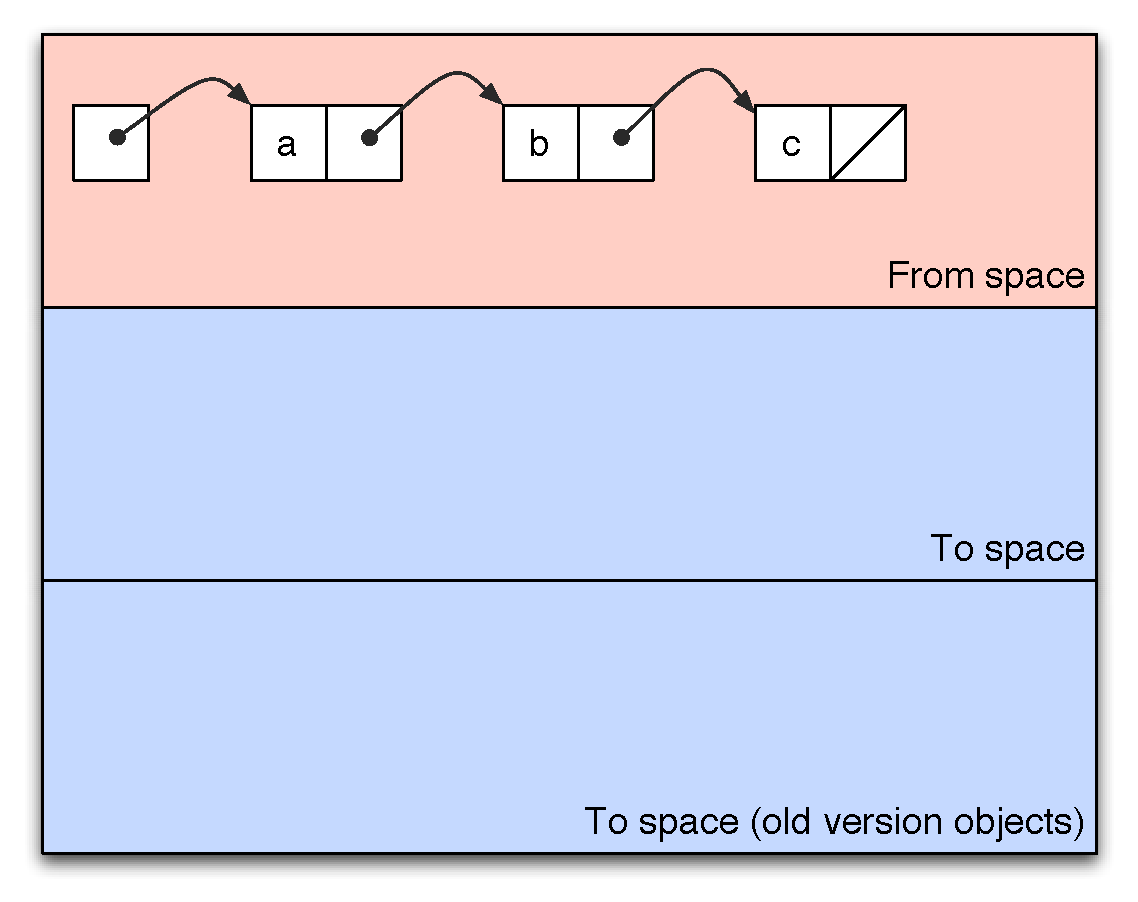
\includegraphics[scale=0.45]{images/singly-doubly/before-gc-copy}}%
\only<2>{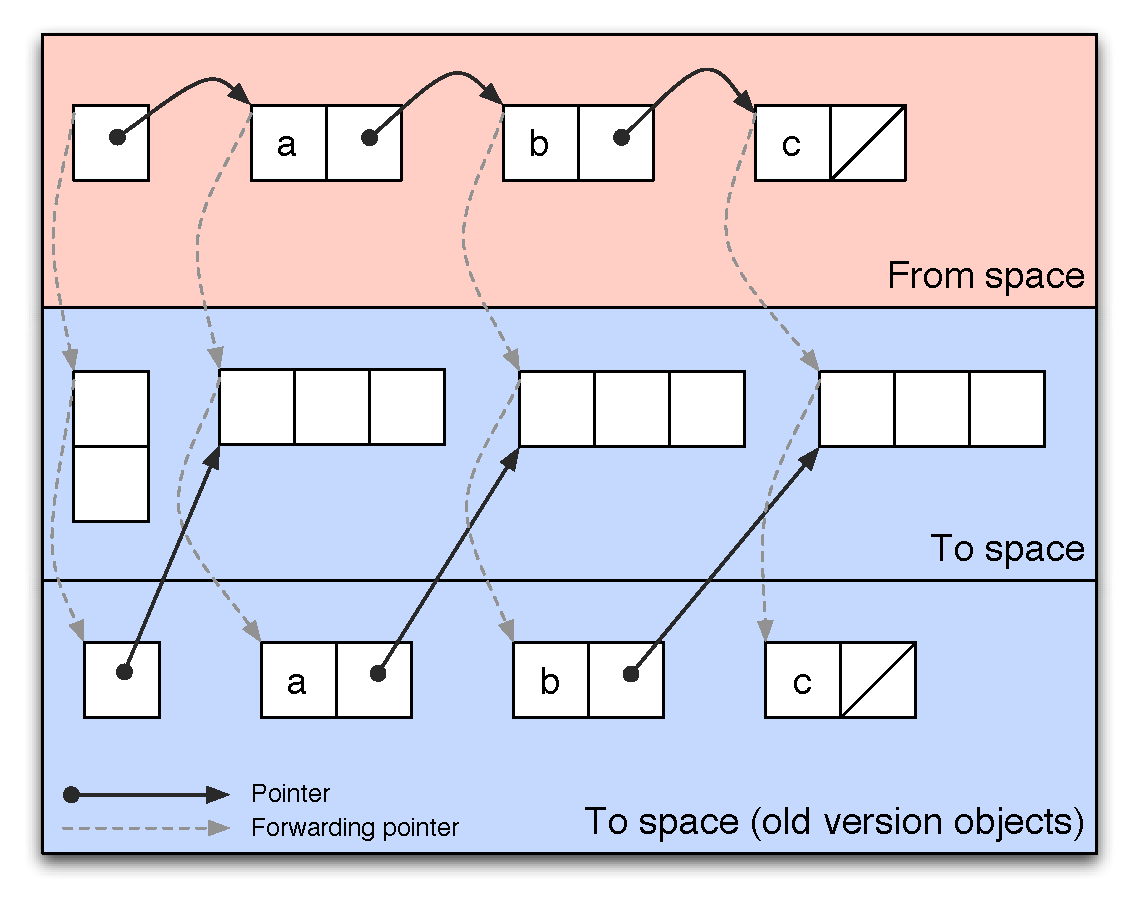
\includegraphics[scale=0.45]{images/singly-doubly/singly-doubly}}%
\only<3>{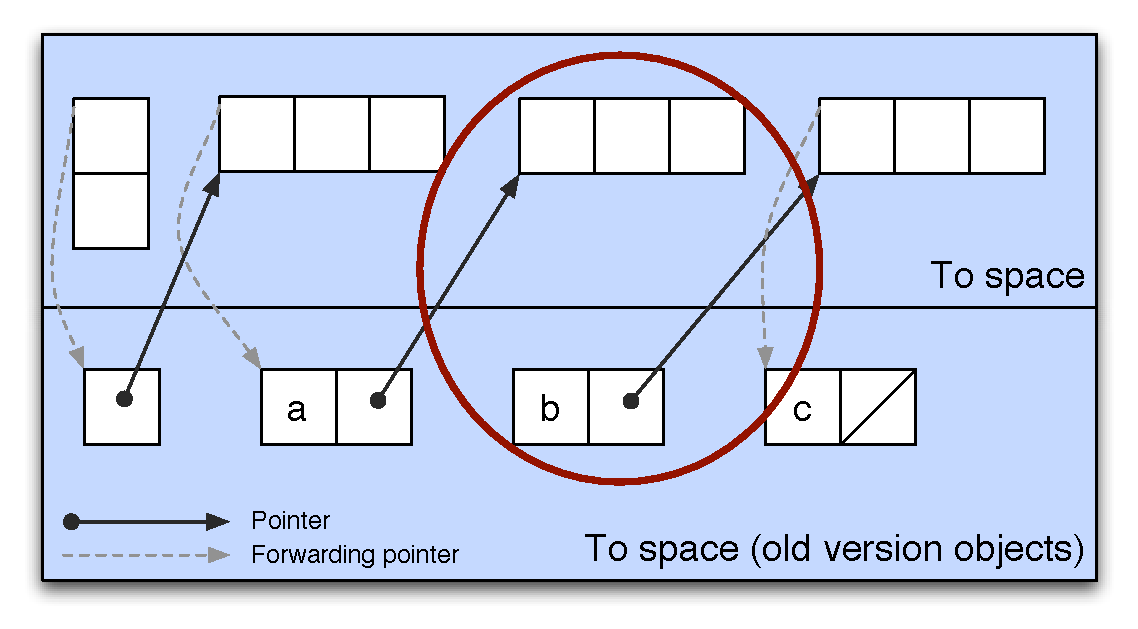
\includegraphics[scale=0.45]{images/singly-doubly/singly-doubly-transform-b-step-0}}
\only<4>{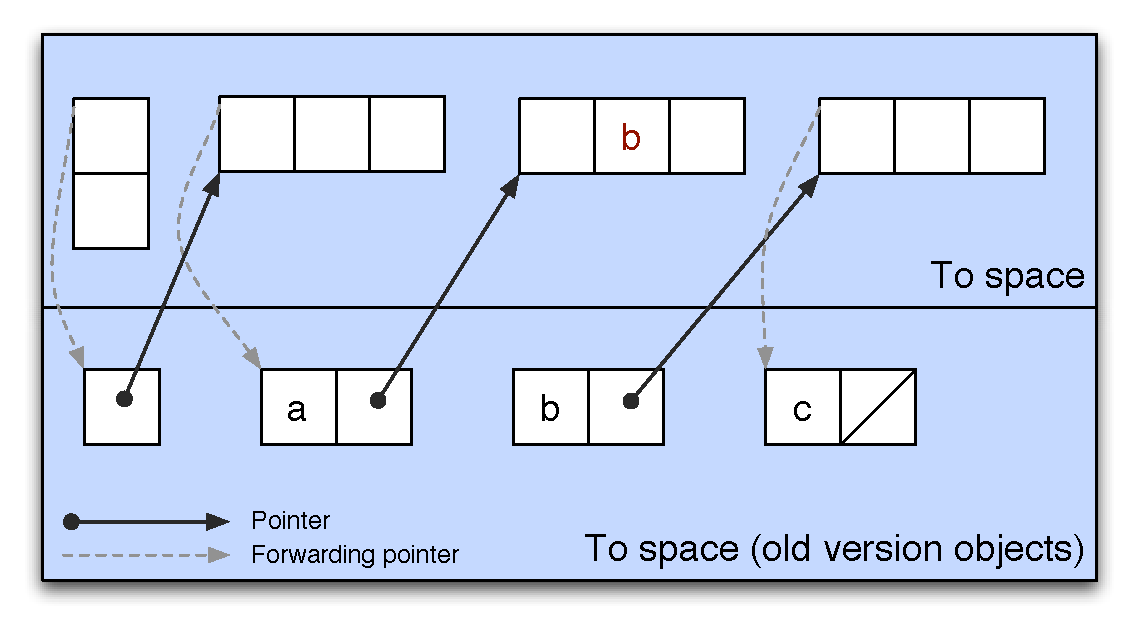
\includegraphics[scale=0.45]{images/singly-doubly/singly-doubly-transform-b-step-1}}
\only<5>{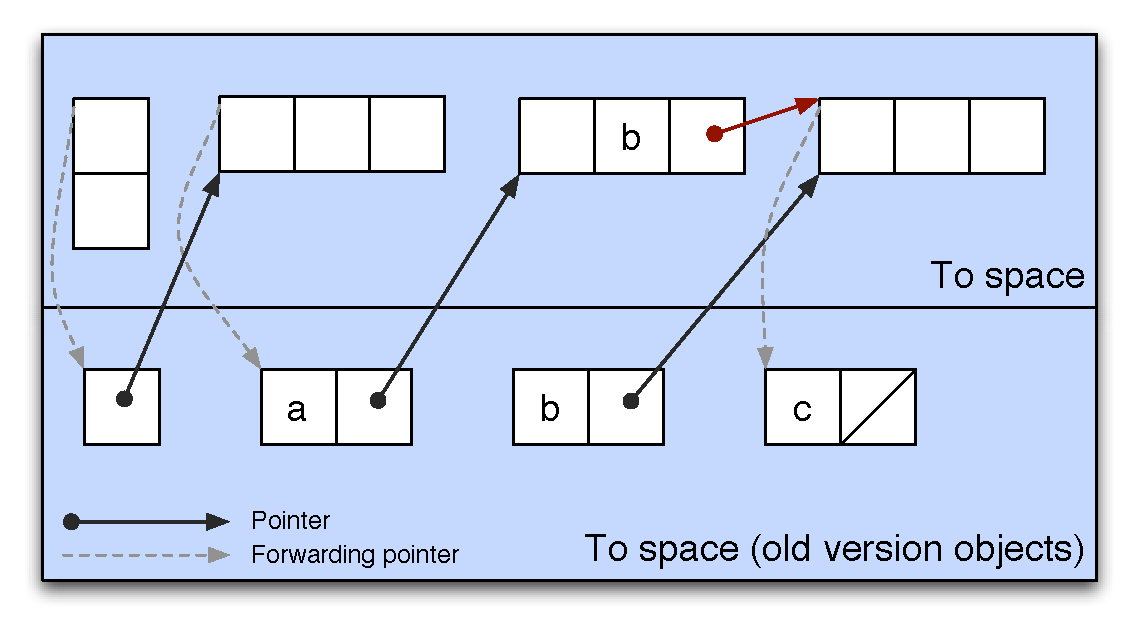
\includegraphics[scale=0.45]{images/singly-doubly/singly-doubly-transform-b-step-2}}
\only<6>{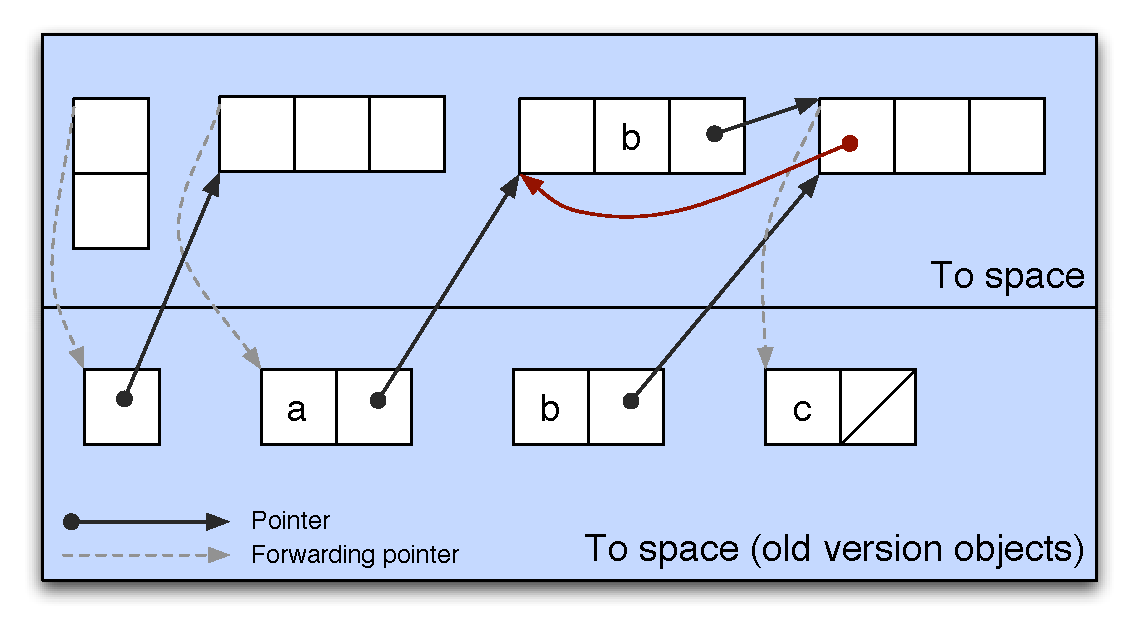
\includegraphics[scale=0.45]{images/singly-doubly/singly-doubly-transform-b-step-3}}
\only<7>{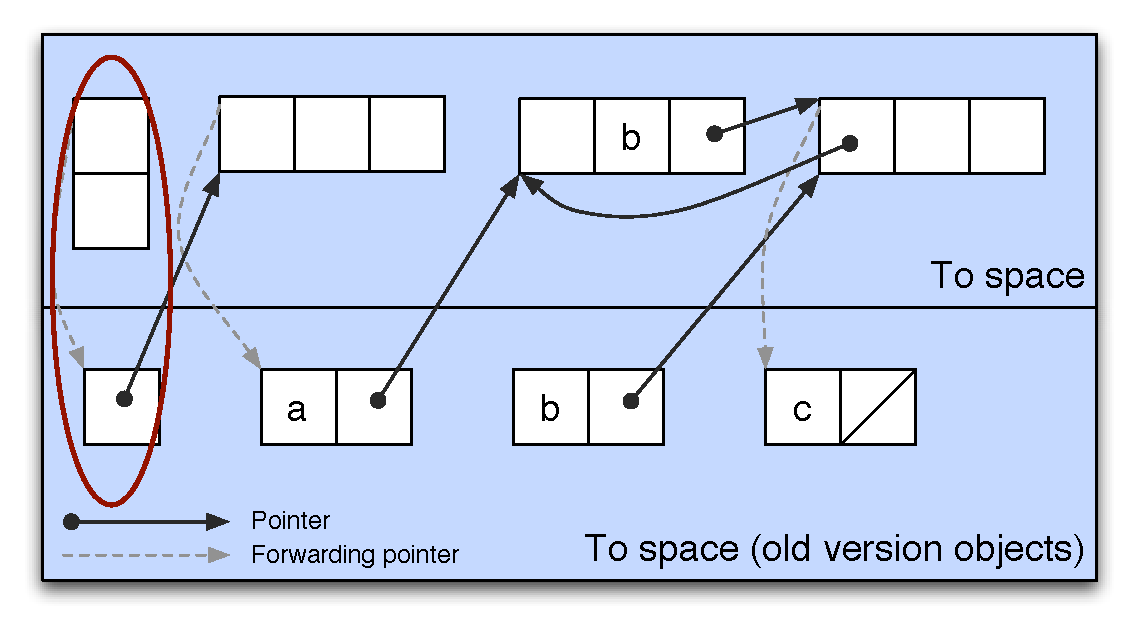
\includegraphics[scale=0.45]{images/singly-doubly/singly-doubly-transform-head-step-0}}
\only<8>{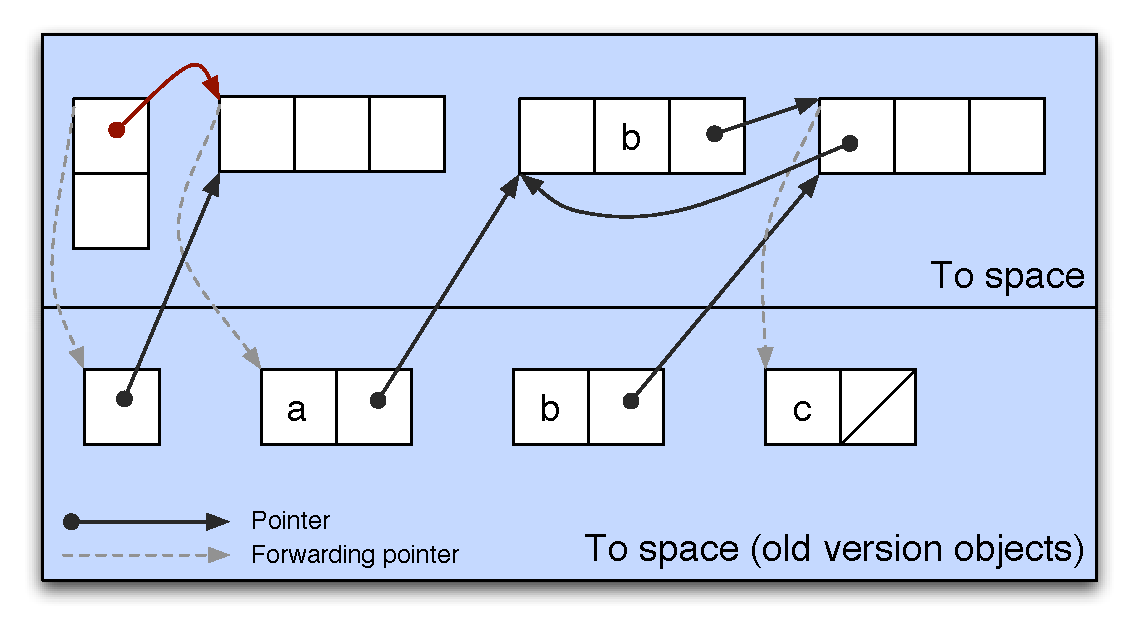
\includegraphics[scale=0.45]{images/singly-doubly/singly-doubly-transform-head-step-1}}
\only<9>{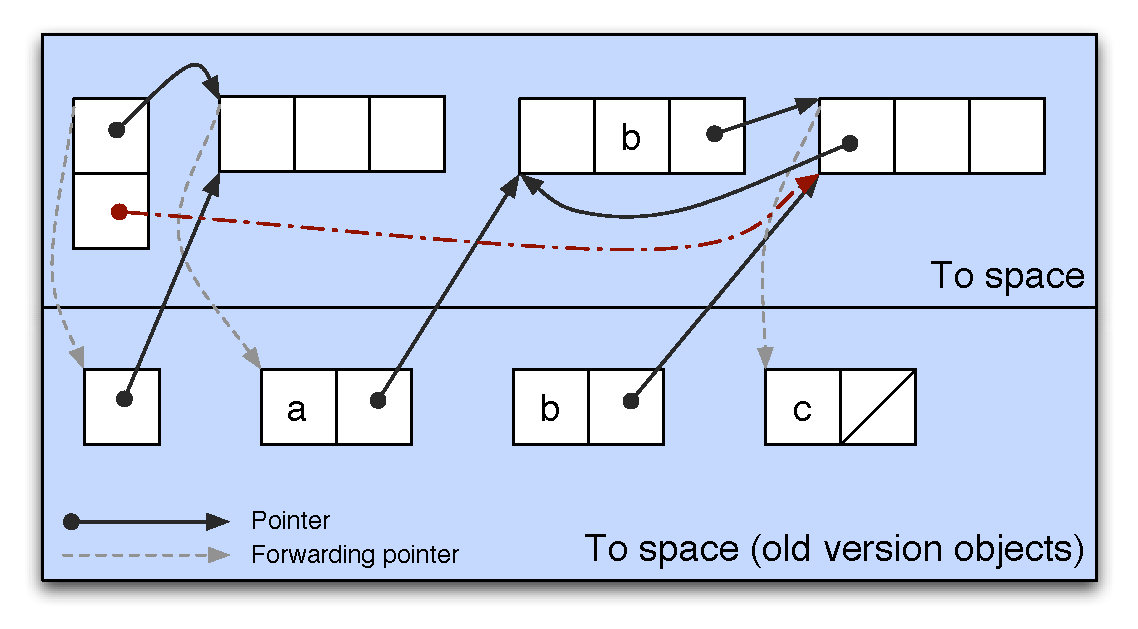
\includegraphics[scale=0.45]{images/singly-doubly/singly-doubly-transform-head-step-2}}
\only<10>{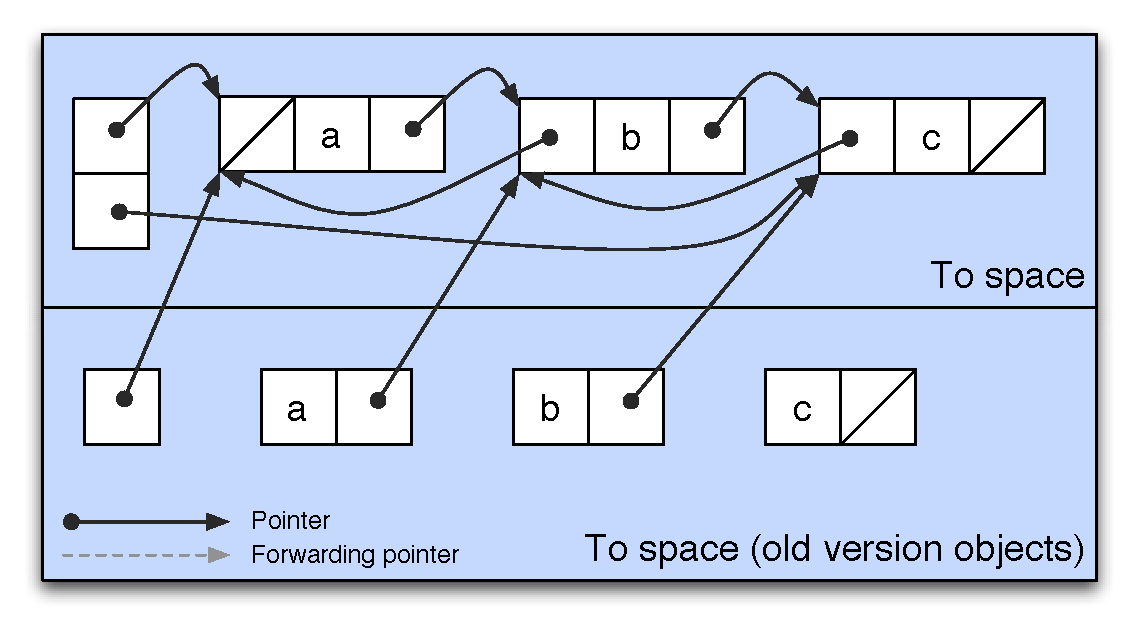
\includegraphics[scale=0.45]{images/singly-doubly/singly-doubly-transformed}}
\only<11>{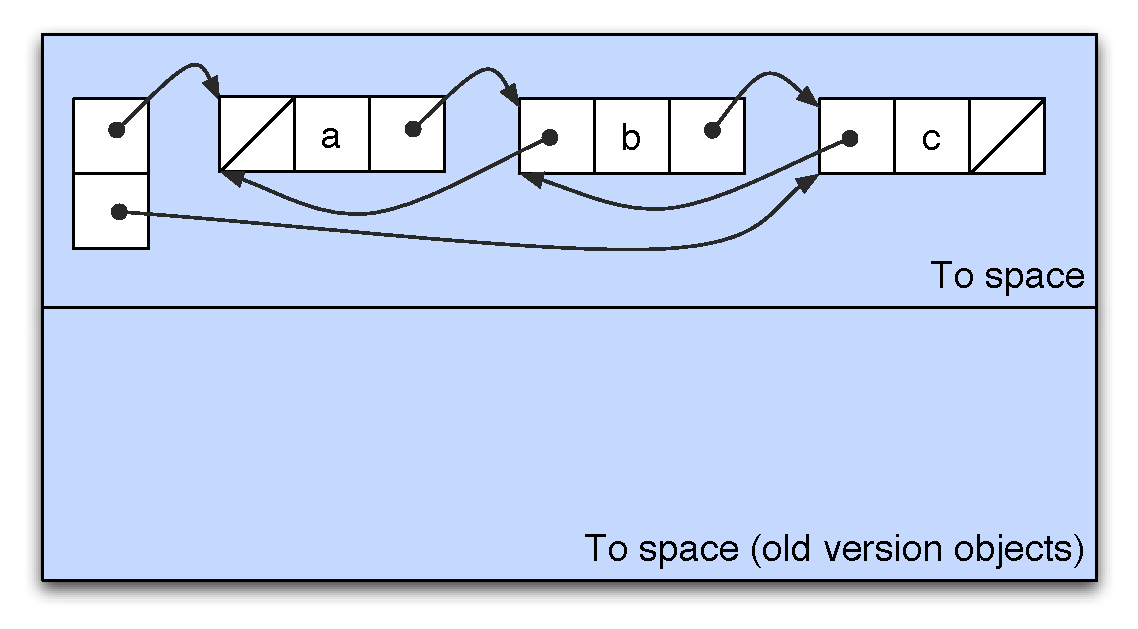
\includegraphics[scale=0.45]{images/singly-doubly/singly-doubly-transformed-final}}
\end{column}
\begin{column}{0.37\paperwidth}%
% Transform b, step 0
\only<3>{%
\begin{footnotesize}%
\noindent {\tt jvolveObject(Node to,}\\
{\tt\ \ \ \ old\_Node from) \{}\\
{\tt\ \ to.data = from.data;}\\
{\tt\ \ to.next = from.next;}\\
{\tt\ \ if (to.next != null)}\\
{\tt\ \ \ \ to.next.prev = to;}\\
{\tt \}}
\end{footnotesize}%
}%
% Transform b, step 1
\only<4>{%
\begin{footnotesize}%
\noindent {\tt jvolveObject(Node to,}\\
{\tt\ \ \ \ old\_Node from) \{}\\
{\tt\ \ \colorbox{yellow}{to.data = from.data;}}\\
{\tt\ \ to.next = from.next;}\\
{\tt\ \ if (to.next != null)}\\
{\tt\ \ \ \ to.next.prev = to;}\\
{\tt \}}
\end{footnotesize}%
}%
% Transform b, step 2
\only<5>{%
\begin{footnotesize}%
\noindent {\tt jvolveObject(Node to,}\\
{\tt\ \ \ \ old\_Node from) \{}\\
{\tt\ \ to.data = from.data;}\\
{\tt\ \ \colorbox{yellow}{to.next = from.next;}}\\
{\tt\ \ if (to.next != null)}\\
{\tt\ \ \ \ to.next.prev = to;}\\
{\tt \}}
\end{footnotesize}%
}%
% Transform b, step 3
\only<6>{%
\begin{footnotesize}%
\noindent {\tt jvolveObject(Node to,}\\
{\tt\ \ \ \ old\_Node from) \{}\\
{\tt\ \ to.data = from.data;}\\
{\tt\ \ to.next = from.next;}\\
{\tt\ \ \colorbox{yellow}{if (to.next != null)}}\\
{\tt\ \ \colorbox{yellow}{\ \ to.next.prev = to;}}\\
{\tt \}}
\end{footnotesize}%
}%
\end{column}
\end{columns}
\end{frame}


% \begin{frame}[t,fragile]{\DSU{} Garbage collector}%{A Sub-title is optional}
% \begin{itemize}
% \item Identical to Semispace for ``regular'' objects
% \item For objects to be transformed
%   \begin{itemize}
%   \item Copy the object to ToSpace (like Semispace)
%   \item Also, allocate an empty object in ToSpace for the new version
%   \end{itemize}
% \item Forwarding pointers point to the ``new version'' object
% \item No field can point to an ``old version'' object
% \end{itemize}
% \end{frame}

% \ifdraft{}{
% % 
%%%%%%%%%%%%%%%%%%%%%%%%%%%%%%%%%%%%%%%%%%%%%%%%%%%%%%%%%%%%%%%%%%%%%%%%
% Now, we show semispace with objects being updated.
%%%%%%%%%%%%%%%%%%%%%%%%%%%%%%%%%%%%%%%%%%%%%%%%%%%%%%%%%%%%%%%%%%%%%%%%
{
\begin{frame}[fragile]{\DSU{} garbage collector}%{A Sub-title is optional}
\setbeamercovered{invisible}
\begin{columns}[t]
\begin{column}[T]{0.67\paperwidth}
\begin{tikzpicture}
\begin{scope}
  % objects
  \uncover<1>{       \node[field] (root) at \objectRoot {root};                        }
  \uncover<2->{      \node[new space black field] (root) at \objectRoot {root};        }
                     \oldSpaceObject{A}{\objectA}
                     \oldSpaceObject{B}{\objectB}
                     \oldSpaceObject[dsu v0 object]{C}{\objectC}
                     \oldSpaceObject{D}{\objectD}
                     \oldSpaceObject{E}{\objectE}
                     \oldSpaceObject[dsu v0 object]{F}{\objectF}
                     \oldSpaceObject{G}{\objectG}
  % forwarding pointers
  \uncover<2->{      \forwardingPointer{A}                             }
  \uncover<3->{      \forwardingPointer{B}
                     \dsuForwardingPointer{C}                          }
  \uncover<4->{      \forwardingPointer{D}
                     \forwardingPointer{E}                             }
  \uncover<5->{      \dsuForwardingPointer{F}
                     \forwardingPointer{G}                             }
  % pointer arrows
  \uncover<1>   {    \path[regular]     (root.east)  to [out=330,in=120] (A.140)    ;          }
  \uncover<1>   {    \path[regular]     (A 0.center) to                (B.90)     ;            }
  \uncover<1>   {    \path[regular]     (A 1.center) to                (C.135)    ;            }
  \uncover<1-2> {    \path[regular]     (B 0.center) to                (D.135)    ;            }
  \uncover<1-2> {    \path[regular]     (B 1.center) to                (E.90)     ;            }
  \uncover<1-2> {    \path[regular]     (C 0.center) to                (F.135)    ;            }
  \uncover<1-2> {    \path[regular]     (C 1.center) to                (G.90)     ;            }
  \uncover<1-4> {    \path[regular]     (F 0.center) to                (A)        ;            }
                                                                      
  \uncover<2> {    \path[transparent]   (root.east)  to [out=0,in=120] (A.140)    ;            }
  \uncover<2> {    \path[transparent]   (A 0.center) to                (B.90)     ;            }
  \uncover<2> {    \path[transparent]   (A 1.center) to                (C.135)    ;            }
  \uncover<3> {    \path[transparent]   (B 0.center) to                (D.135)    ;            }
  \uncover<3> {    \path[transparent]   (B 1.center) to                (E.90)     ;            }
  \uncover<3> {    \path[transparent]   (C 0.center) to                (F.135)    ;            }
  \uncover<3> {    \path[transparent]   (C 1.center) to                (G.90)     ;            }
  \uncover<5> {    \path[transparent]   (F 0.center) to                (A)        ;            }

  \draw[draw,thin] (-4,-2.5) rectangle (4,0.5);
  \draw (4,0.5) node[anchor=north east,inner sep=1pt,font=\tiny] {FromSpace};

\end{scope}
\begin{scope}[yshift=-3.75cm]
  % objects
  \uncover<2>   {    \newSpaceGreyObject{A'}{\objectAprime}                          }
  \uncover<3->  {    \newSpaceBlackObject{A'}{\objectAprime}                         }

  \uncover<3>   {    \newSpaceGreyObject{B'}{\objectBprime}                          }
  \uncover<4->  {    \newSpaceBlackObject{B'}{\objectBprime}                         }

  \uncover<3-4> {    \dsuNewSpaceGreyObject{C'}{\objectCprime}                       }
  \uncover<5-10>{    \dsuNewSpaceBlackObject{C'}{\objectCprime}                      }
  \uncover<3->  {    \newSpaceVersionOneEmptyObject{C'}{\objectCprimeVersionOne}     }

  \uncover<4-5> {    \newSpaceGreyObject{D'}{\objectDprime}                          }
  \uncover<6->  {    \newSpaceBlackObject{D'}{\objectDprime}                         }

  \uncover<4-6> {    \newSpaceGreyObject{E'}{\objectEprime}                          }
  \uncover<7->  {    \newSpaceBlackObject{E'}{\objectEprime}                         }

  \uncover<5-7> {    \dsuNewSpaceGreyObject{F'}{\objectFprime}                       }
  \uncover<8-10>{    \dsuNewSpaceBlackObject{F'}{\objectFprime}                      }
  \uncover<5->  {    \newSpaceVersionOneEmptyObject{F'}{\objectFprimeVersionOne}     }

  \uncover<5-8> {    \newSpaceGreyObject{G'}{\objectGprime}                          }
  \uncover<9->  {    \newSpaceBlackObject{G'}{\objectGprime}                         }

  % pointer arrows
  \uncover<2->  {    \path[regular] (root.west)   to [out=220,in=95] (A'.north west);    }
  \uncover<2>   {    \path[regular] (A' 0.center) to [out=130,in=180] (B.west);
                     \path[regular] (A' 1.center) to [out=70,in=180]  (C.west);           }
  \uncover<3->  {    \path[regular] (A' 0.center) to [out=80,in=135]  (B'.150);          
                     \path[regular] (A' 1.center) to [out=270,in=110] (C' v1.north west); }
                                                                                         
  \uncover<3>   {    \path[regular] (B' 0.center) to                  (D.south);         
                     \path[regular] (B' 1.center) to                  (E.south);          }
  \uncover<4->  {    \path[regular] (B' 0.center) to [out=300,in=240] (D'.215);          
                     \path[regular] (B' 1.center) to [out=330,in=240] (E'.215);           }
                                                                                         
  \uncover<3-4> {    \path[regular] (C' 0.center) to                  (F.south);         
                     \path[regular] (C' 1.center) to                  (G.south west);     }
  \uncover<5-10>{    \path[regular] (C' 0.center) to [out=255,in=105]  (F' v1.north west);          
                     \path[regular] (C' 1.center) to [out=70,in=150]  (G'.150);           }
                                                                                         
  \uncover<5-7> {    \path[regular] (F' 0.center) to [out=30,in=325]  (A);                }
  \uncover<8-10>{    \path[regular] (F' 0.center) to [out=215,in=330] (A'.215);           }

  % transparent arrows
  \uncover<3>   {    \path[transparent] (A' 0.center) to [out=130,in=180] (B.west);
                     \path[transparent] (A' 1.center) to [out=70,in=180]  (C.west);       }

  \uncover<4>   {    \path[transparent] (B' 0.center) to                  (D.south);
                     \path[transparent] (B' 1.center) to                  (E.south);      }

  \uncover<5>   {    \path[transparent] (C' 0.center) to                  (F.south);
                     \path[transparent] (C' 1.center) to                  (G.south west); }

  \uncover<8>   {    \path[transparent] (F' 0.center) to [out=30,in=325]  (A);            }

  % v1 arrows
  \uncover<10-> {    \path[regular] (C' v1 0.center) to [out=30,in=120]   (F' v1.north west);
                     \path[regular] (C' v1 1.center) to                   (G'.210);          
                     \path[regular] (F' v1 0.center) to [out=180,in=315]  (A'.215);
                }
  

  \draw[draw,thin] (-4,-2) rectangle (4,0.5);
  \draw (4,-2) node[anchor=south east,inner sep=1pt,font=\tiny] {ToSpace};
\end{scope}
\end{tikzpicture}
\end{column}
\begin{column}[T]{0.25\paperwidth}
\begin{block}{}
\begin{tikzpicture}
\tikzstyle{column 2}=[anchor=west]
\matrix [row sep=0.5ex] {
\node[dsu v0 field] {};          & \node {\tiny To be transformed}; \\
\node[dsu v1 empty field] {};    & \node {\tiny $v_1$ object}; \\
};
\end{tikzpicture}
\end{block}

\begin{block}{}
\begin{footnotesize}
\only<1>{
The same heap as before. Objects to be transformed are highlighted.
}
\only<2>{
Copy A.
}
\only<3>{
Scan A'. Copy B and C. In addition an empty object C'$v_1$ is allocated.
\alert{A' points to this copy and not the old one.}
}
\only<4>{
Scan B'.
}
\only<5>{
Scan C'.
}
\only<6>{
Scan D'.
}
\only<7>{
Scan E'.
}
\only<8>{
Scan F'.
}
\only<9>{
GC is now complete. No field can point to C'$v_0$ or F'$v_0$. Pointers to C and
F point to $v_1$ (empty) objects. \texttt{memcpy(v\_1, v\_0);} will give us a valid
heap.}
\only<10>{
Setting fields of C'$v_1$ and F'$v_1$.
}
\only<11>{
C'$v_0$ and F'$v_0$ can be reclaimed.
}
\end{footnotesize}
\end{block}
\end{column}
\end{columns}
\end{frame}
}

% vim:tw=0:nospell

% {
\begin{frame}[fragile]{\DSU{} Garbage collector}%{A Sub-title is optional}
\setbeamercovered{invisible}
\begin{center}
\begin{tikzpicture}
  % objects
                  \node[field] (root) at \objectRoot {root};
                  \oldSpaceObject{A}{\objectA}
                  \oldSpaceObject{B}{\objectB}
\uncover<-2>{     \dsuOldSpaceVersionZeroObject{C}{\objectC}                  }
                  \oldSpaceObject{D}{\objectD}
                  \oldSpaceObject{E}{\objectE}
\uncover<-2>{     \dsuOldSpaceVersionZeroObject{F}{\objectF}                  }
                  \oldSpaceObject{G}{\objectG}

                  \dsuOldSpaceVersionOneObject{C}{\objectCVersionOne}
                  \dsuOldSpaceVersionOneObject{F}{\objectFVersionOne}

                  % pointer arrows
                  \path[regular]     (root.east)  to [out=330,in=120]     (A.140);
                  \path[regular]     (A 0.center) to                      (B.90);
                  \path[regular]     (A 1.center) to                      (C v1.190);
                  \path[regular]     (B 0.center) to                      (D.135);
                  \path[regular]     (B 1.center) to                      (E.90);
\uncover<-2>{     \path[regular]     (C 0.center) to [out=180,in=90]      (F v1.north west);
                  \path[regular]     (C 1.center) to                      (G.90);
                  \path[regular]     (F 0.center) to                      (A);                       }

\uncover<2-3>{    \path[regular]     (C v1 0.center) to [out=180,in=120]  (F v1.north west);
                  \path[regular]     (C v1 1.center) to                   (G.60);
                  \path[regular]     (F v1 0.center) to                   (A);                       }

  \draw[draw,thin] (-4,-3.5) rectangle (4,0.5);
\end{tikzpicture}
% \begin{block}{}
% Loren ipsum. Hello World. Hello World. Hello World.  Loren ipsum. Hello World.
% Hello World. Hello World.  Loren ipsum. Hello World. Hello World. Hello World.
% Loren ipsum. Hello World.\footnote{This is a footnote} Hello World. Hello World.  Loren ipsum. Hello World.
% Hello World. Hello World.
% \end{block}
\end{center}
\end{frame}
}

% vim:tw=0:nospell

% % {
\begin{frame}[fragile]{Revisiting transformation functions}%{A Sub-title is optional}
\setbeamercovered{invisible}
\begin{center}
\begin{tikzpicture}
  % objects
  \node[field] (root) at \objectRoot {root};
  \oldSpaceObject{A}{\objectA}
  \oldSpaceObject{B}{\objectB}
  \dsuOldSpaceVersionZeroObject{C}{\objectC}
  \oldSpaceObject{D}{\objectD}
  \oldSpaceObject{E}{\objectE}
  \dsuOldSpaceVersionZeroObject{F}{\objectF}
  \oldSpaceObject{G}{\objectG}
  \dsuOldSpaceVersionOneObject{C}{\objectCVersionOne}
  \dsuOldSpaceVersionOneObject{F}{\objectFVersionOne}

  % pointer arrows
  \path[regular]     (root.east)  to [out=330,in=120]     (A.140);
  \path[regular]     (A 0.center) to                      (B.90);
  \path[regular]     (A 1.center) to                      (C v1.190);
  \path[regular]     (B 0.center) to                      (D.135);
  \path[regular]     (B 1.center) to                      (E.90);
  \path[regular]     (C 0.center) to [out=180,in=90]      (F v1.north west);
  \path[regular]     (C 1.center) to                      (G.90);
  \path[regular]     (F 0.center) to                      (A);

  \draw[draw,thin] (-4,-3.5) rectangle (4,0.5);
\end{tikzpicture}
\begin{block}{We have an ordering problem}
\texttt{(C $v_0$).field0.field0} might be uninitialized
\end{block}
\end{center}
\end{frame}
}

% vim:tw=0:nospell

% }

% \begin{frame}[t,fragile]{Revisiting transformation functions}%{A Sub-title is optional}
% Solutions to the ordering problem \\
% \begin{itemize}
% \item Programmer can invoke a VM function that will transform objects on
% demand. Moves burden of safety to the programmer
% \uncover<2>{
% \item Insert read barrier code to perform this check when compiling the
% transformation function
% \item Perform some static analysis to determine an order to queue
% objects
% }
% \end{itemize}
% \end{frame}

\section{Experience}
\label{sec:experience}

To evaluate \DSU, we used it to update three open-source servers written
in Java: the Jetty webserver\footnote{\url{http://www.mortbay.org}},
JavaEmailServer,\footnote{\url{http://www.ericdaugherty.com/java/mailserver/}}
an SMTP and POP e-mail server, and CrossFTP server.\footnote{\url{http://www.crossftp.com/}}
These programs belong to a class that
should benefit from DSU because they typically run continuously. DSU
would enable deployments to incorporate bug fixes or add new features
without having to halt currently-running sessions.  

We explored
updates corresponding to releases made over roughly one to two years
of each program's lifetime.  Of the 22 updates we considered, \DSU{} could
support 20 of them---the two updates we could not apply changed
classes with infinitely-running methods, and thus no safe point could
be reached.  To our knowledge, no existing DSU system
for Java could support all these updates; indeed, previous systems
with simple support for updating method bodies would be able to handle only 9 of the 22 updates.  Although \DSU{} cannot support every
update, it is the first DSU system for Java
that has been shown to support changes to realistic programs as they
occur in practice over a long period of time.

In the rest of this section, we first examine the performance impact of
\DSU{}, and then look at updates to each of the three applications in
detail.

\input{experience/performance-jetty-table}
\input{experience/performance-microbench-table}

\subsection{Performance}
\label{subsec:performance}

The main performance impact of \DSU{} is the cost of applying an update;
once updated, the application eventually runs without further overhead.  To confirm
%MWH: added "eventually" here because of the cost of recompilation.
%We don't actually measure this though.  Is that a problem?
this claim, we measured the throughput and latency of two Jetty versions while running on
stock \JikesRVM{} and on \DSU{} after dynamically updating to the next version. The performance of these configurations is
essentially identical.

% We report
% on this experiment in Section~\ref{subsec:jetty-perf}.

The cost of applying an update is the time to load any new classes, invoke a
full heap garbage collection, and to apply the transformation methods on
objects belonging to updated classes.
Roughly,
the time to suspend threads and check
that the application is in a safe-point is less than a millisecond, and classloading
time is usually less than 20ms.
% (Classloading could occur in parallel with normal execution.) 
Therefore the update disruption time is primarily
due to the GC and object transformers, and is proportional
to the size of the heap and the fraction of objects being transformed.  We
wrote a simple microbenchmark to measure these overheads.
% Section~\ref{subsec:microbench}
This experiment shows that object
transformation is the dominant cost.

We conducted all our experiments on an Intel Core 2 Quad machine running at 2.4 GHz machine with 2 GB of RAM.
The machine ran Ubuntu 7.10 on Linux kernel version 2.6.22. We implemented
\DSU{} on top of \JRVMVersion{}.

% We also have microbenchmarks where we compare the
% overhead added as a result of running the transformer function.

\input{experience/performance-jetty}
\input{experience/performance-microbench}


\newcommand{\ChangedClassesColumn}{third}
\begin{table}
\begin{footnotesize}
\begin{center}
\begin{tabular}{|l||c||c|c|c|r|c|c|} \hline \T
Ver.    & \#      & \multicolumn{6}{c|}{\# changed} \\
        & classes & \multicolumn{1}{c|}{classes} & \multicolumn{3}{c|}{methods} & \multicolumn{2}{c|}{fields} \\
        & added   &         & add & del & \multicolumn{1}{c|}{chg}             & add & del \\ \hline \hline \T
5.1.1   & 0       & 14      &\ 4  & 1   &  38/0            &  0  & 0   \\
5.1.2   & 1       &\ 5      &\ 0  & 0   &  12/1            &  0  & 0   \\
5.1.3*  & 3       & 15      & 19  & 2   &  59/0            & 10  & 1   \\
5.1.4   & 0       &\ 6      &\ 0  & 4   &   9/6            &  0  & 2   \\
5.1.5   & 0       & 54      & 21  & 4   & 112/8            &  5  & 0   \\
5.1.6   & 0       &\ 4      &\ 0  & 0   &  20/0            &  5  & 6   \\
5.1.7   & 0       &\ 7      &\ 8  & 0   &  11/2            &  9  & 3   \\
5.1.8   & 0       &\ 1      &\ 0  & 0   &   1/0            &  0  & 0   \\
5.1.9   & 0       &\ 1      &\ 0  & 0   &   1/0            &  0  & 0   \\
5.1.10  & 0       &\ 4      &\ 0  & 0   &   4/0            &  0  & 0   \\ \hline
\end{tabular}
\end{center}
\end{footnotesize}
\caption{Summary of updates to Jetty}
\label{tab:jetty-changes}
\end{table}

\subsection{Jetty webserver}
\label{subsec:jetty}

Jetty is a popular webserver written in Java. It supports static
and dynamic content and can be embedded 
within other Java applications. \JikesRVM, and thus \DSU, is not able to run the
most recent versions of Jetty (6.x).  Therefore we considered 11
versions, consisting of 5.1.0 through 5.1.10 (the last version prior to
version 6).  Version 5.1.10 contains 317 classes and about 45,000 lines
of code.  Table~\ref{tab:jetty-changes} shows a summary of the changes
in each update.  Each row tabulates the changes relative
to the prior version. For the column listing changed methods, the
notation $x/y$ indicates that $x+y$ methods were changed, where $x$
changed in body only, and $y$ changed their type signature as well.
For dynamic updating systems that only support changes to method
bodies, only the first and last three of the ten updates could be
supported, since the rest either change method signatures
and/or add or delete fields.

\paragraph{Reaching a safe point in Jetty.}
We  successfully wrote dynamic updates to all
versions of Jetty that we examined. For each version starting at 5.1.0, we ran
Jetty under full load. After 30 seconds we tried to apply the update to the
next version. We did this five times per version.  Other than the
update to 5.1.3, all versions immediately 
reached a safe point every time, with no need of return barriers.

We could not apply the update to version 5.1.3 (denoted with an
asterisk in the table) 
because \DSU{} was never able to reach a safe point. The update modified
{\tt ThreadedServer.accept\-Socket()}, a method that waits for a connection
from the client, and this method is nearly always on stack. 
We installed a return barrier that is triggered when {\tt
  acceptSocket} returns, but this barrier is not sufficient to perform the
update since the main methods of several threads were themselves
modified. For example, we also install a return barrier on {\tt
  Pool\-Thread.run()}, but this barrier is never triggered because
this method never becomes inactive.

% REFACTOR: add para back if we get things to work.
% We refactored the various long-running main methods in versions 5.1.2 and
% 5.1.3 to extract the modified bodies of long running methods into separate
% methods and leave the main method containing the loop unmodified between
% the two versions.  (This sort of transformation is performed by other
% systems automatically by programmer directive in
% Ginseng~\cite{neamtiu06dsu}.) 
% When we attempted to perform a dynamic update, \DSU{}
% installed a return barrier for {\tt acceptSocket()}. This function waits
% for a connection and returns after a timeout. \DSU{} was able to update the
% application when this function returned. 

% To understand why, we instrumented the VM to emit information about
% restricted method set and, if a safe point cannot be reached, which
% restricted method was active. 

% \suriya{The following information about inlining is commented out. What
% should we do with this? See .tex file}
%     For each version, starting at 5.1.0, we
%     ran Jetty under full load.  After 30 seconds we tried to apply the
%     update to the next version; if a safe point could not be immediately
%     reached, we deemed the attempt as failed.
%     The results are presented in
%     Table~\ref{tab:inlining}.  Column 2 shows the number of times out of
%     five such runs where the application reached a safe point.  The methods
%     whose presence on a thread stack precluded the application from
%     reaching a safe point are mentioned below the table.  For the update to
%     5.1.3, the offending method was always active because it contained an
%     infinite loop.  The other updates either always succeeded, or did after a
%     small number of retries.
%     
%     Column 3 contains the total number
%     of methods in the program at runtime, where the number in parentheses is the
%     number of those which the compiler inlined when using aggressive
%     optimization.
%     This provides an upper bound on the effect of inlining in reaching a
%     safe point.  The next group of columns contains the restricted method
%     set. Each column in the group specifies the number of methods loaded at
%     run time by the VM, followed by the total number of methods in that
%     category in the program. The first column in this group is the number of methods in
%     classes involved in a class update. Recall that when a class is updated, say by adding
%     a field, all its methods are considered restricted (see section~\ref{sec:safe}).
%     \suriya{Provide reference to where we explain restricted. and redefine
%     restricted}
%     The second column in this group is the number of methods whose
%     bodies are updated, the third is the number of methods
%     indirectly updated, and the fourth sums these, with the number of methods
%     that were inlined written in parentheses. % The first and second
%     % columns in this group together constitute all the methods of classes that
%     % were changed, as enumerated in the \ChangedClassesColumn{} column in table~\ref{tab:jetty-changes}.
%     The final two columns list
%     the total number of methods in the restricted set; they differ from the
%     first number in the fourth column by the number of (transitively)
%     inlined callers of the restricted methods that were not already
%     restricted.  The final column uses \DSU{}'s OSR analysis to determine the
%     number of restricted methods although OSR itself was not applied.
%     
%     The table shows that both indirect method calls \suriya{or updates?} and inlining significantly
%     add to the size of the restricted set.  Inlining though, is small by
%     comparison, because all callers of an updated class's methods are
%     \emph{already} included in the indirect set. Therefore, inlining these
%     methods adds no further restriction.
%     In most cases OSR support would dramatically reduce the number of
%     restricted methods and increase the likelihood of reaching a DSU safe
%     point.
%     Interestingly, having a greater number of restricted methods overall
%     does not necessarily reduce the likelihood that an update will take
%     effect; rather, it depends on the frequency with which methods in this
%     set are on the stack.

%%% Local Variables: 
%%% mode: latex
%%% TeX-master: "../pldi64"
%%% End: 

\subsection{JavaEmailServer}
\label{subsec:jes}

\begin{table}[t]
\begin{footnotesize}
\begin{center}
\begin{tabular}{|l||c|c||c|r|c|r|r|c|} \hline \T
Ver.   & \multicolumn{2}{c||}{\# classes} &    \multicolumn{6}{c|}{\# changed} \\
       & add & del & classes & \multicolumn{3}{c|}{methods} & \multicolumn{2}{c|}{fields} \\
       &     &     &         & add & del & chg   & add & del \\ \hline \hline \T
1.2.2  & 0   & 0   & 3       & 0   & 0   & 3/0   & 0   & 0   \\
1.2.3  & 0   & 0   & 7       & 0   & 0   & 14/2  & 12  & 0   \\
1.2.4  & 0   & 0   & 2       & 0   & 0   & 4/0   & 0   & 0   \\
1.3*   & 4   & 9   & 2       & 11  & 3   & 6/9   & 12  & 5   \\
1.3.1  & 0   & 0   & 2       & 0   & 0   & 4/0   & 0   & 0   \\
1.3.2  & 0   & 0   & 8       & 4   & 2   & 4/2   & 3   & 1   \\
1.3.3  & 0   & 0   & 4       & 0   & 0   & 3/0   & 0   & 0   \\
1.3.4  & 0   & 0   & 6       & 2   & 0   & 6/0   & 2   & 0   \\
1.4    & 0   & 0   & 7       & 6   & 1   & 4/1   & 6   & 0   \\ \hline
\end{tabular}
\end{center}
\end{footnotesize}
\caption{Summary of updates to JavaEmailServer}
\label{tab:jes-changes}
\end{table}

For JavaEmailServer, we considered 10 versions---1.2.1 through
1.4---spanning a duration of about two years.   Version 1.4 
consists of 20 classes and about 5000 lines of code. 
Table~\ref{tab:jes-changes} shows the summary of changes for each new
version. Approaches that only support updates to method bodies will be able
to handle only four of these updates. We
could successfully construct updates for all versions we examined, and
we could successfully apply all of them except the update to version 1.3.
This update reworks the configuration framework of the server, among other
things removing a GUI tool for user administration and adding several
new classes that implement a file-based configuration system.  As a result, many of
the classes are modified to point to a new configuration object.
Among these classes are threads with infinite processing loops (e.g., to accept
POP and SMTP requests). Because these threads are always active, the
safety condition can never be met and thus the update cannot be
applied.

The update from 1.3.1 to 1.3.2 indirectly changes the
\texttt{SMTP\-Sen\-d\-er.run()} and \texttt{Pop3\-Processor.run()} methods.  These
methods contain processing loops run by several threads.  Though these
methods are always running, \DSU{} applies OSR and the update succeeds.
\DSU{} also uses OSR for the update from 1.3.2 to 1.3.3.
%MWH: suriya says this statement just isn't true.  Updates fine.
% A method used to process connections was also changed, and this method
% is frequently active when the server is under load.  (A similar
% method was changed in the update to version 1.3.3.)  A return barrier
% installed on this method permits the update to take effect.  

\begin{table}[t]
\begin{footnotesize}
\begin{center}
\begin{tabular}{|l||c|c||c|c|c|r|c|c|} \hline \T
Ver.   & \multicolumn{2}{c||}{\# classes} &    \multicolumn{6}{c|}{\# changed}             \\
       & add & del & classes & \multicolumn{3}{c|}{methods} & \multicolumn{2}{c|}{fields}  \\
       &     &     &         & add & del & chg   & add & del                               \\ \hline \hline \T
1.06   & 4   & 1   & 1       & 0   & 0   & 3/0   & 1   & 0                                 \\
1.07   & 0   & 0   & 3       & 4   & 0   & 14/0  & 5   & 0                                 \\
1.08   & 0   & 1   & 3       & 2   & 0   & 10/0  & 0   & 2                                 \\ \hline
\end{tabular}
\end{center}
\end{footnotesize}
\caption{Summary of updates to CrossFTP server}
\label{tab:crossftp-changes}
\end{table}

\subsection{CrossFTP server}
\label{subsec:crossftp}
CrossFTP server is an easily configurable, security-enabled FTP server.
CrossFTP allows simple configuration through a GUI and more advanced
customization using configuration files. We did not use the GUI interface
and therefore do not consider changes to that part of the program.  We
looked at 4 versions--- 1.05 through 1.08, details shown in Table~\ref{tab:crossftp-changes}---spanning a duration of more
than a year. Version 1.08 contains about 18,000 lines of code spread across
161 classes. \DSU{} successfully applies all three updates to this
application.  Note that since all updates either add or delete fields,
simple method body updating support on its own would be insufficient.

\DSU{} could only apply the update from version 1.07 to 1.08 when the
server was relatively idle.
%MWH: I added relatively here, since the update should work when there
%is one connection, by our explanation: i.e., one thread running
%RequestHandler.run() will hit its return barrier and the update takes
%place.  Maybe two connections too, if you get lucky, etc.
The server runs a new {\tt RequestHandler} thread to process each FTP
session, and the \texttt{RequestHandler.run()} method was changed by
the update.   \DSU{} installs a return barrier on this method,
but with many active sessions, this method is essentially always on stack,
preventing the update.  Future work could address this problem using scheduler support
for coordinating updates among active threads~\cite{neamtiu09stump}.


\section{Future Work}
\ShowTOC
\begin{frame}{Looking ahead}%{A Sub-title is optional}
\begin{center}
\begin{Huge}
What's in the path towards mainstream adoption?
\end{Huge}
\end{center}
\end{frame}

\begin{frame}{Safety}%{A Sub-title is optional}
\begin{itemize}
\item Currently, we guarantee type safety. Can we do more?
\item Safe behavior in a general context is undecidable \cite{Gupta94}
\item Divide program into transactions, ensure they are version consistent
\cite{neamtiu08context}
\item Exhaustively testing updates
\end{itemize}
\end{frame}

\begin{frame}{Flexibility}%{A Sub-title is optional}
\begin{itemize}
\item Supporting every possible update is not a goal
\item Support most of the updates that occur in practice
\item Large and complex applications and updates
\item Understand update semantics from refactorings
\end{itemize}
\end{frame}

\begin{frame}{Efficiency}%{A Sub-title is optional}
\begin{itemize}
\item Update time roughly proportional to GC time
\item Semi-space GC is not practical
\item We have two requirements
  \begin{itemize}
  \item Copying objects
  \item Full-heap collection
  \end{itemize}
\item Other collectors? Concurrent collectors?
\end{itemize}
\end{frame}

\section{Conclusion}
% \ShowTOC

% \begin{frame}{Future work}%{A Sub-title is optional}
% \begin{itemize}
% \item Baby steps towards using static analysis towards asserting safety of
% updates
% \item Restricting update points based on semantics of the update
% \item How can we show that these update points are indeed safe?
% \end{itemize}
% \end{frame}

\begin{frame}{Conclusion}%{A Sub-title is optional}
\begin{itemize}
\item \DSU{}, a Java VM with support for Dynamic Software Updating
\item Most-featured, best-performing DSU system for Java
\item Naturally extends existing VM services
\item Supports about two years worth of updates
\end{itemize}
\begin{block}{}
\emph{Dynamic software updating in managed languages can be achieved in a
safe, flexible and efficient manner.}
\end{block}
\begin{center}
Source code and other information:
\url{http://www.cs.utexas.edu/~suriya/jvolve}
% Also available in the Jikes
% RVM research archive.
\end{center}
\end{frame}

% \begin{frame}{Research plan}%{A Sub-title is optional}
% \begin{center}
% \begin{large}
% Bridge the gap between static and dynamic languages
% \end{large}
% \end{center}
% \begin{itemize}
% \item Static Languages: Java, C\#
%   \begin{itemize}
%   \item Compile-time type safety
%   \item Static analysis
%   \item High performance VMs
%   \end{itemize}
% \item Dynamic Languages: Python, Ruby
%   \begin{itemize}
%   \item Expressive
%   \item Concise programs, easy to write/understand
%   \item No compile-time guarantees
%   \end{itemize}
% \end{itemize}
% \begin{center}
% \begin{large}
% Improved safety and performance of Dynamic languages
% \end{large}
% \end{center}
% \end{frame}
% 
% \begin{frame}{Solutions}%{A Sub-title is optional}
% \begin{itemize}
% \item Diamondback Ruby: Static type checking for Ruby
% \item Languages targeting the JVM: Clojure, Groovy, etc.
% \item Dynamic Language VMs: Unladen Swallow, PyPy
% \item Gradual typing
% \item DaVinci project: Dynamic language support in JVM
% \item Static Typing Where Possible, Dynamic Typing When Needed
% \end{itemize}
% \end{frame}
% 
% \begin{frame}{Conclusion}%{A Sub-title is optional}
% \begin{itemize}
% \item Work towards improving the robustness of software systems
% \item Current work: A VM-based Dynamic Software Updating solution
% \item In the future: Robust Dynamic Languages
% \end{itemize}
% \end{frame}

\appendix
\begin{frame}[allowframebreaks]{References}%{A Sub-title is optional}
\bibliographystyle{apalike}
\bibliography{paper.bib}
\end{frame}



\end{document}
